\documentclass[12pt,a4paper, openright]{book}

\usepackage[left=3.5cm,top=2.5cm,right=2.5cm,bottom=2.5cm]{geometry} %margins
\usepackage{amsthm} % theorem environment
\usepackage{amsmath} % math
\usepackage{amssymb} % symbols
\usepackage{graphics} % for including figures
\usepackage{graphicx} % for including figures
\usepackage{setspace} % for doublespacing singlespacing etc.
\usepackage{datetime} % to write the date in the desired format
\usepackage[title, titletoc]{appendix}
\usepackage{subfigure}
\usepackage{algorithm}
%\usepackage{algorithmic}
\usepackage{longtable}
\usepackage{bm}
\usepackage{verbatim}
\usepackage{algorithmicx}
\usepackage{algpseudocode}
\usepackage{float}
\usepackage{listings}
\usepackage{framed}
\usepackage{multirow}
\usepackage{booktabs}
\usepackage{chngpage}
%\usepackage[square, comma, sort&compress]{natbib}
\usepackage[numbers]{natbib}
\usepackage{hyperref}
\usepackage{fixltx2e}
\usepackage{url}
\usepackage{pdfpages}
\usepackage{caption}
\usepackage{tikz}
\usepackage{afterpage}

%\usepackage{subcaption}
%\usepackage{hyperref}
%\usepackage{afterpage}
\usepackage{fancyhdr}

\theoremstyle{definition}
\newtheorem{example}{Example}
\newtheorem{definition}{Definition}
\newtheorem{proposition}{Proposition}

\DeclareMathOperator*{\argmax}{arg\,max}
\newcommand{\todo}[1]{\textcolor{red}{\textbf{TODO:} #1}}
\newcommand{\setD}{\ensuremath{\mathbf{D}} }
\newcommand{\setW}{\ensuremath{\mathbf{V}} }
\newcommand{\setC}{\ensuremath{\mathbf{C}} }
\newcommand{\matD}{\ensuremath{\mathrm{D}} }
\newcommand{\matW}{\ensuremath{\mathrm{W}} }
\newcommand{\matC}{\ensuremath{\mathrm{C}} }
\newcommand{\vecdi}[1]{\ensuremath{\mathrm{v}^{D}_{#1}}}
\newcommand{\vecwi}[1]{\ensuremath{\mathrm{v}^{W}_{#1}}}
\newcommand{\vecci}[1]{\ensuremath{\mathrm{v}^{C}_{#1}}}
\newcommand{\con}{$(w_{t-c}, \ldots, w_{t-1}, w_{t+1}, \ldots, w_{t+c})$}
\newcommand{\wgt}[1]{\ensuremath{\lambda_{#1}}}
\newcommand{\traindata}{\ensuremath{\mathcal{T}}}
\newcommand{\db}{\ensuremath{\mathcal{D}} }
\newcommand{\para}[1]{\noindent\textbf{%\fontsize{14}{15}\selectfont 
#1}} %{\paragraph{#1}}
\newcommand{\highest}[1]{\textbf{#1}}

\newcommand\blankpage{%
    \null
    \thispagestyle{empty}%
    %\addtocounter{page}{-1}%
    \newpage}


\graphicspath{{figs/}}

\pagestyle{myheadings} 

%\setlength{\LTpre}{0pt}
\setlength{\LTpost}{-40pt}
\setlength{\LTcapwidth}{\textwidth}
% % % % % % % % % % % % % % % % %

%all this for generating title and certificate
\newdateformat{monthyear}{\monthname[\THEMONTH], \THEYEAR}
\def\title{Learning Distributed Document Representations for Multi-Label Document Categorization}
\def\subtitle{}
\def\author{Nitish Gupta}
\def\rollno{10327461}
\def\degree{B.Tech. - M.Tech. (Dual Degree)}
\def\department{Department of Electrical Engineering}
\def\shortdepartment{EE}
\def\institute{Indian Institute of Technology Kanpur}
\def\shortinstitute{I.I.T. Kanpur}
\def\longinstitute{Indian Institute of Technology, Kanpur}
\def\advisormain{Prof. Harish Karnick}
\def\advisorsec{Prof. Rajesh M. Hegde}
\def\advisormaindepartment{Department of Computer Science and Engineering}
\def\advisorsecdepartment{Department of Electrical Engineering}
\def\instituteaddress{Kanpur-208016}

% % % % % % % % % % % % % % % % % 

\hypersetup{
	bookmarks=true,
	bookmarksopen=true,
	bookmarksopenlevel=0,
	bookmarksnumbered=true,
	hypertexnames=false,
	colorlinks=true,
	linkcolor={black},
	citecolor={black},
	urlcolor={black},
	breaklinks=true,
	pdfauthor={\author},
	pdftitle={\title}
}


\begin{document}
	\frontmatter
	
\includepdf{title.pdf}

	\thispagestyle{empty}
	\pagestyle{plain}
	\cleardoublepage
    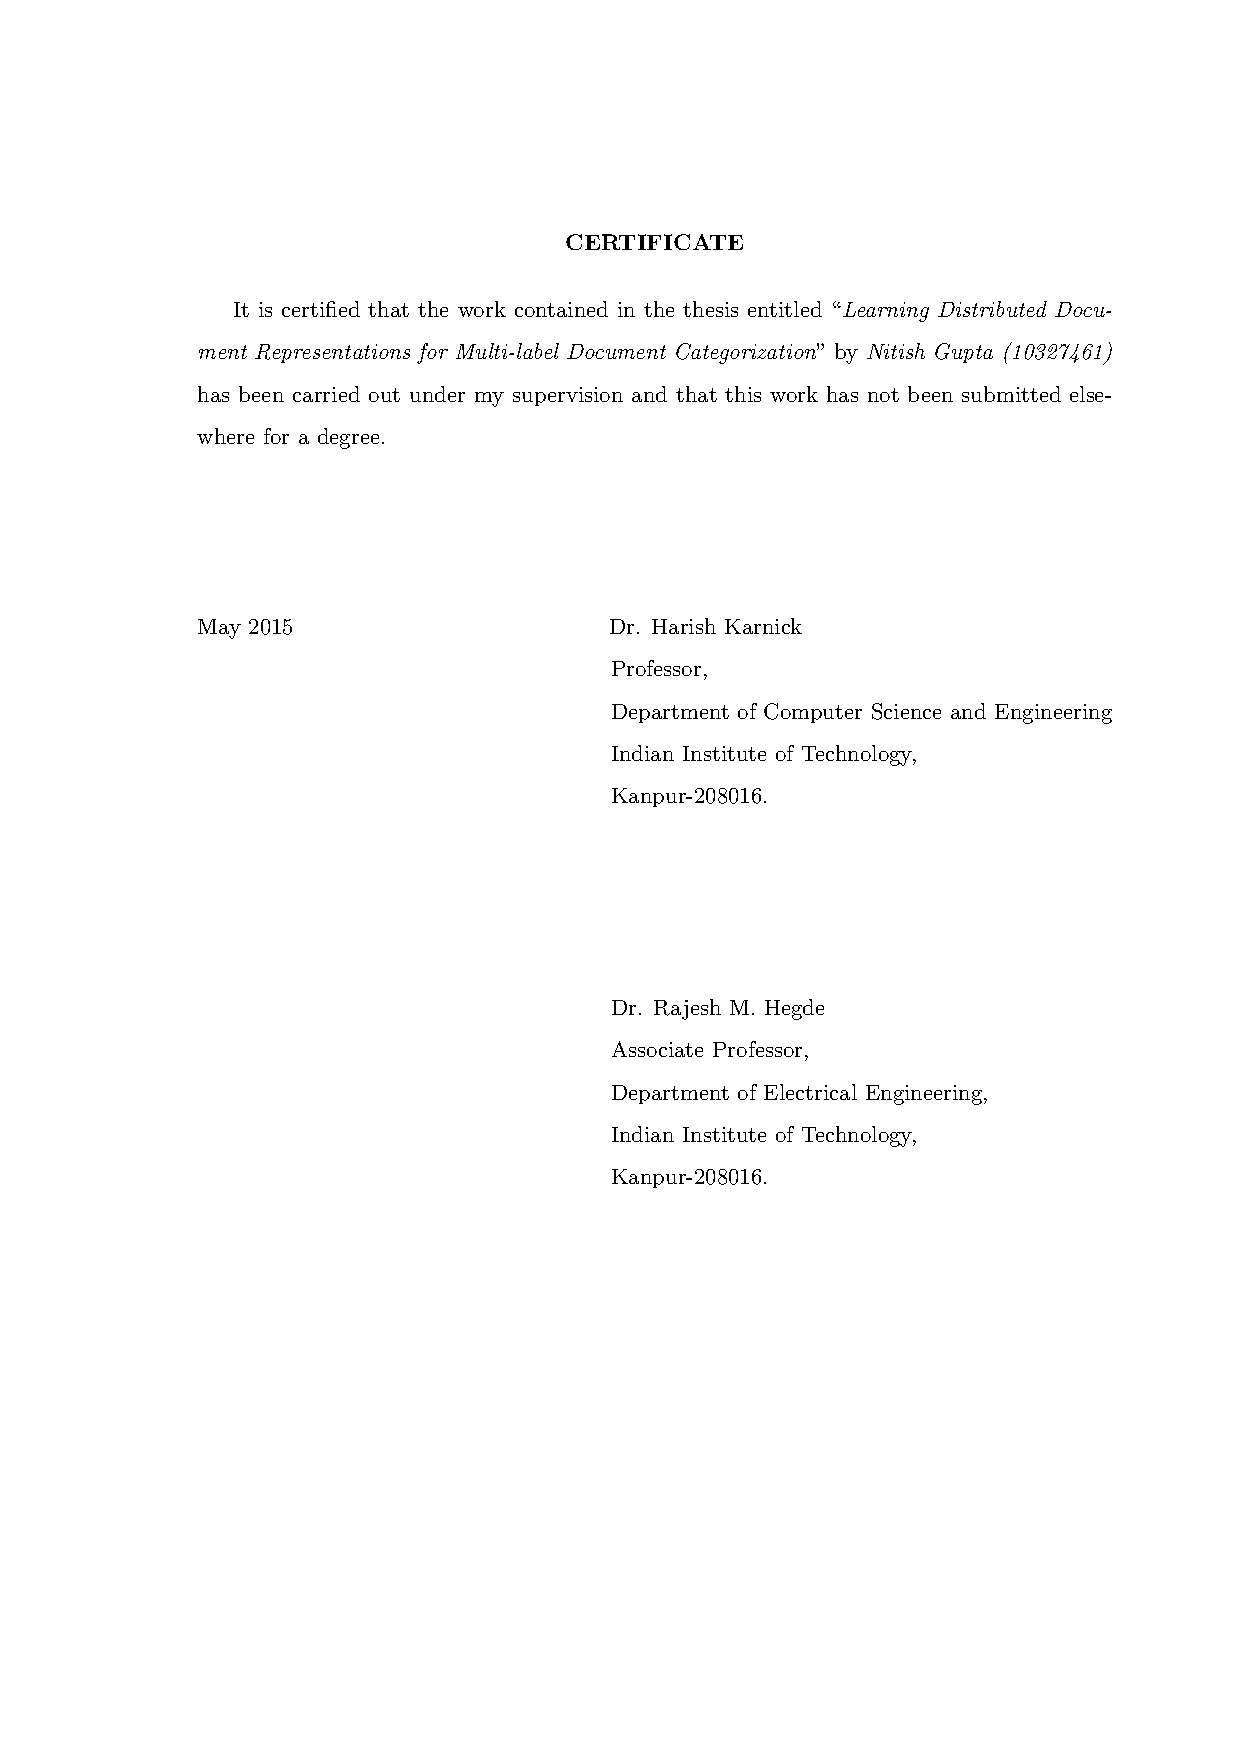
\includepdf{certificate.pdf}
    \blankpage


	\pagenumbering{roman} 
	\pagestyle{plain}
	\setcounter{page}{5}
	\addcontentsline{toc}{chapter}{Abstract}
	
	\onehalfspace
	\begin{center}
\huge{\textbf{Abstract}}
\end{center}

% Multi-label Document Categorization, the task of automatically assigning a text document into one or more categories is a crucial step in knowledge management and has various real-world applications such as categorizing news articles, tagging Web pages, maintaining medical patient records and organizing digital libraries among many others. 
% Statistical Machine Learning approaches to document categorization have focused on multi-label learning algorithms such as Support Vector Machines, k-Nearest Neighbors, Logistic Regression, Neural Networks, Naive Bayes, Generative Probabilistic Models etc. while the input to such algorithms i.e. the vector representation for documents has traditionally been used as the bag-of-words representation model. 
% %The input to such algorithms i.e. the vector representation for documents has traditionally been used as the bag-of-words representation model due to its simplicity and ability to capture the topical content of the documents.
% Though the usage of simple bag-of-words document representation gives surprisingly accurate results, it suffers from sparsity, high-dimensionality and lack of similarity measures along with various drawbacks such as the inability to preserve word ordering and contextual information in which the words occur in the documents. Encoding contextual information about words in documents is crucial to capture the correct semantic content of the highly complex and ambiguous human language.  \hfill \break

% Our work is focused on learning continuous distributed vector representations for documents by embedding all the documents in the same low-dimensional space such that documents that are similar in their semantic content have similar vector representations. To tackle the issues in bag-of-words representation model, we present an unsupervised neural network model that, given a word in a document, uses the document representation along with the contextual information in which the word occurs, to predict it and learn document representations along with learning distributed word vectors. 
% %By learning low-rank distributed representations and incorporating contextual information in which the words occur in the documents we try to overcome the drawbacks posed by the bag-of-words representations. 
% We use a modified version of the logistic regression algorithm to learn similar distributed representations for categories to perform the document categorization task. As we embed documents, categories and words in the same low-dimensional space, estimating similarity between them is as simple as taking a dot-product between the vectors of the entities. We show that the representations learned using our model give state-of-the-art results in the document categorization task on standard \emph{Reuters-21578} and Wikipedia datasets and also show promising results in imputing missing categories in existing articles on Wikipedia against the bag-of-words representations.
Multi-label Document Categorization, the task of automatically assigning a text document into one or more categories has various real-world applications such as categorizing news articles, tagging Web pages, maintaining medical patient records and organizing digital libraries among many others. Statistical Machine Learning approaches to document categorization have focused on multi-label learning algorithms such as Support Vector Machines, k-Nearest Neighbors, Logistic Regression, Neural Networks, Naive Bayes, Generative Probabilistic Models etc. while the input to such algorithms i.e. the vector representation for documents has traditionally been used as the bag-of-words model. Though the usage of simple bag-of-words representation gives surprisingly accurate results, it suffers from sparsity, high-dimensionality, lack of similarity measures along with other drawbacks such as the inability to encode word ordering and contextual information in which the words occur. Encoding contextual information about words in documents is crucial to capture the correct semantic content of the highly complex and ambiguous human language.  \hfill \break

Our work is focused on learning continuous distributed vector representations for documents by embedding all the documents in the same low-dimensional space such that documents that are similar in their semantic content have similar vector representations. To tackle the issues in bag-of-words representation model, we present an unsupervised neural network model that uses the document vector to predict words in the document along with using the contextual information in which the word occurs and jointly learns distributed document and word representations. We use a modified version of the logistic regression algorithm to learn similar distributed representations for categories to perform the document categorization task. We show that the representations learned using our model give state-of-the-art results in the document categorization task on the standard \emph{Reuters-21578} and Wikipedia datasets and also show the effectiveness of our model in imputing missing categories in existing articles on Wikipedia against the bag-of-words representations. As we embed categories and words in the same low-dimensional space we can also estimate similarities between them which is not directly observed in the data. We qualitatively demonstrate that the learned representations are also able to capture the semantic dependencies between categories and words. 
	\blankpage
	
\vspace*{\fill}

\begin{center}
%{\it Dedicated to my parents and my brother}\\
{\it Dedicated to}\\
{\it My Family}
\end{center}

\vspace*{\fill}

	\blankpage
	\begin{center}
	{\huge{\textbf{Acknowledgement}}}
\end{center}
I wouldn't like to express my sincere gratitude towards my thesis supervisor, {\advisormain}, for his constant support and encouragement. I am grateful for his patient guidance and advice in giving a proper direction to my efforts. I am also grateful to {\advisorsec} for giving me the freedom to work on a topic of my liking.

\paragraph*{}
Last, but not the least, I would like to thank my parents and brother for their love and encouragement. Without their support and patience this work would not have been possible. 

\vskip 4mm
\begin{flushright}
\textit{\textbf{\author}}
\end{flushright}





	\blankpage

	\doublespacing
    \setcounter{secnumdepth}{3}
	\setcounter{tocdepth}{1}
	\tableofcontents
	\listoftables
	\addcontentsline{toc}{chapter}{List of Tables}
	
	\listoffigures
	\addcontentsline{toc}{chapter}{List of Figures}
	
	\listofalgorithms
	\addcontentsline{toc}{chapter}{List of Algorithms} 
		
	\mainmatter
	\doublespacing
	\pagenumbering{arabic}
	\pagestyle{myheadings}
	
	\chapter{Introduction}
\label{chapter:introduction}

\todo{ Section 2 : Problem Statement. Formally with document vectors $x_{d_{i}}$ and task of finding appropriate label vector $l_{d_{i}}$ Section. Along with table as in http://lpis.csd.auth.gr/publications/tsoumakas-ijdwm.pdf 3 : Contribution Section 4 : Organization of thesis}

Text documents usually belong to more than one conceptual class. For example, a document on music piracy can be simultaneously classified into \emph{Arts/Music}, \emph{Internet/Security}, \emph{Laws/Cyber}.     Multi-Label Document Categorization \emph{(also known as Text Categorization or Classification)} is the task of assigning a text document to one or more pre-defined categories to describe the semantic content of a document and provide a conceptual view of the document collection.
With the growth of online information, Document Categorization has found its use in many important real world applications ranging from document organization to information retrieval. It can be used to organize news stories by categories (topics), classify academic papers by the technical domains and sub-domains they belong to, cluster documents based on their semantic content for easy retrieval and recommendation etc.
With the advent of crowd-sourced databases such as Wikipedia\footnote{www.wikipedia.org} which contains over $4$ million documents that are manually categorized from a category set containing over $500$ thousand categories, automatic document categorization is utmost necessary and useful to assign categories to new articles that are added on a daily basis and also assign missing categories to older documents.

The task of multi-label classification belongs to a general family of supervised learning where the training instances along with the labels they belong to are used to learn a multi-label classifier that assigns appropriate labels to new test instances. 
Another supervised learning task that is very relevant to multi-label classification is that of \emph{ranking}. In the ranking task, the learning algorithm learns a ranking function from the training examples that ranks the set of labels for a new instance such that the more relevant labels are the topmost in the ranked list. 
To generate the proper output of the multi-label classifier, i.e. the set of relevant labels for the test instance, post-processing of the ranked list of categories is required.

Supervised machine learning techniques that learn classifiers to perform the document categorization task can be broken down into two main components, namely, text representation and learning algorithm. 
Text representation involves converting the documents, that are usually strings of characters, into numerical vectors that are suitable inputs to the learning algorithm while the learning algorithm uses pairs of labeled input text representations and the categories it belongs to, to learn a model so as to assign relevant categories to new documents. \todo{ADD COMPLETE SYTEM FIGURE.}

Over the years, documents have been represented as a \emph{bag-of-words} feature vector, which contains information about the presence and absence of words in the document. Given a corpus of documents, each document $d_{i}$ in the corpus is represented as a vector $v_{d_{i}} \in \mathbb{R}^{|V|}$ whose size is equal to the size of the vocabulary. Each element in the vector belongs to $\{0, 1\}$ and denotes whether the particular word is present in the document or not. Though bag-of-words document representation has been widely used for document categorization due to its simplicity, efficiency and ability to capture topical content of the documents necessary for categorization, it suffers from various drawbacks. Bag-of-words representation ignores word ordering and the context in which the words appear in the document, that is vital for encoding the semantic content of text. It also lacks in the ability to encode the semantic similarity between words and documents to estimate distances between them. Disadvantages of such sought have necessitated the need for a more robust and efficient document representation model.
%In the section below we describe the drawbacks of the bag-of-words model and why there is a need for an alternate document representation model.

Models to learn fixed-length continuous distributed word vector representations from huge corpora of unlabeled text have shown promising results in tasks of language modeling \citep{bengio2003neural}, sentiment analysis \citep{socher2013recursive}, machine translation \citep{zou2013bilingual} etc. by supplementing the labeled data to overcome the inherent data sparsity and improving generalization accuracies in the high-dimensional domain of Natural Language Processing. Such models learn low-dimensional (generally of the order $100$ - $500$) vector representations of words that encode the semantic similarity between them \citep{mikolov2013efficient}. 

Though these word embeddings try to overcome disadvantages of the bag-of-words model, it is unclear how thy can be composed to represent continuous text, namely documents. In this work we present a model to learn such low-dimensional distributed vector representations for documents to aid in the task of document categorization.
 
\section{Motivation}

\subsection{Inability to preserve word ordering}
The prime drawback faced by the bag-of-words representation is their inability to preserve word ordering information in the text. Language is a complex phenomenon that often changes meaning when the word ordering in sentences changes, even though they may contain exactly the same words. For example, even though the sentences
\begin{quote}
\centering
\emph{ 	Jim can only ride bicycles. } and \emph{ 	Only Jim can ride bicycles. }
\end{quote}
contain exactly the same words and hence have the same bag-of-words representation, they completely differ in their meaning. While the first sentence points to the fact that \emph{Jim} only rides bicycles among other vehicles, the second sentence suggests that no one apart from \emph{Jim} knows how to ride a bicycle. 
Similarly, the phrases 
\begin{quote}
\centering
\emph{ 	``a good book'' } and \emph{ 	``book a good'' }
\end{quote}
that have the same bag-of-words representations though they contain different topical content. A document containing the first phrase would like by categorized under \emph{Literature} while containing the second under \emph{Trade}.
As shown in the examples above, document representations that preserve word ordering and information about the context the words occur in are more likely to perform better at the task of document categorization.

\subsection{Lack of similarity measures}
Distance or similarity between two documents is commonly computed by taking the dot product of their corresponding representation vectors. In the case of bag-of-words representation, this amounts to counting the number of words co-occurring in the two documents. For example, consider the case when all the words in a document $d_{1}$ are replaced by synonyms to form another document $d_{2}$, in one case, and replaced by random words to form $d_{3}$ in another. The distance between vectors of $d_{1}$ and $d_{2}$ will be exactly the same as the distance between vectors of $d_{1}$ and $d_{3}$ even though $d_{1}$ and $d_{2}$ are much closer to each other than to $d_{3}$. 
Hence, the other major issue faced by the bag-of-words representations is the lack of ability to encode semantic similarity between words and documents. 
This problem can be partially tackled with the aid of an external Lexical Knowledge Database, such as WordNet for the English Language though an ideal representation should internally encode semantic similarity.

Along with the above stated problems, bag-of-words representations also suffer from high-dimensionality and sparsity issues due to huge vocabulary size in large-scale document corpora that may contain upto million unique words.

\subsection{Compositionality of distributed word vectors}
Though word vectors have shown their efficacy in lot of different NLP tasks, they are limited in their ability to express the meaning of longer phrases and sentences. Document Categorization as a task requires the document representation to encode all the semantic topics present in the document for accurate categorization. There has been progress towards learning distributed representations of documents but it limited to simple weighted average of word vectors. Though it deals with the problem of sparsity and high-dimensionality present in the bag-of-words representation, the problem of preserving word order and contextual information still stands.

In this work, we present an unsupervised model for learning distributed vector representations of documents that along with encoding semantic content of the document also tries to incorporate the contextual information surrounding the words in the document.

\section{Problem Statement}	
Given a set of documents ....

\section{Contributions of Thesis}

\section{Organization of Thesis}








	\chapter{Related Work}
\label{chapter:relatedwork}
The task of text classification, i.e. classification of documents into a fixed number of predefined categories has been long studied in-depth for many years now. This multi-class classification problem has further evolved into a multi-label text classification task where each document can belong to multiple, exactly one or no category at all. 

Supervised machine learning techniques that learn classifiers to perform this category assignment task can be broken down into two main components, namely, text representation and learning algorithm. 
Text representation involves converting the documents, that are usually strings of characters, into numerical vectors that are suitable inputs to the learning algorithm while the learning algorithm uses pairs of labeled input text representations and the categories it is belongs in, to learn a model so as to classify new documents into categories.

\section{Text Representation}
\label{sec:textrepr}
Any text-based classification system requires the documents to be represented in an appropriate manner dictacted by the task being performed \citep{lewis1992text}. Moreover, \citep{quinlan1983learning} showed that the accuracy of the classification task depends as much on the document representation as on the learning algorithm being employed. Different from the data mining task, which deals with structureed documents, text classification deals with unstructured documents that need to be appropriately transformed into numerical vectors, i.e. the need for text representation. In this section we introduce the most effective and widely-used techniques to represent documents for text classification.

\subsection{Bag of Words}
It is found in information retrieval research that word stems work well as representations units for documents and that their ordering in a document is of minor importance for many tasks. This is attributed by the fact that the most widely-used used model to represent documents for the classification task is the \emph{Vector Space Model (VSM)} \citep{salton1973specification}. 

In the Vector Space Model, a document $d$ is represented as a vector in the term/word space, $d$ $=$ $(w_{1}, w_{2}, \ldots, w_{|V|})$ where $|V|$ is the size of the vocabulary. Each of the $w_{i} \in \left[0,1\right]$, represents the weightage of the term $i$ in the document $d$. This is called the \emph{bag-of-words} model as it ignores word ordering and each document is reduced to a bag of words that it contains or not. 

An important requirement of such a representation is that, the terms that help in defining the semantic content of the document and play an important role in classification be given higher weightage than the others. Over the years, there has been much research in the information retrieval field on term weighting schemes. The most important term-weighting techniques are described below : 
\begin{enumerate}
\item{\textbf{One Hot Representation} : }This is the most trivial representation, where each document is represented by a vector that is size of the vocabulary. Each element in the vector is either a $0$ or a $1$ to denote the absence or presence of a specific term in the document.

\item{\textbf{Term Frequency (tf))} : }The term frequency representation weighs the terms present in the document relative to their occurence frequency in the document. Hence a document $d$ is represented as, $d$ $=$ $(w_{1}, w_{2}, \ldots, w_{|V|})$, where, $w_{k}$ is the number of times the term $k$ appears in the document $d$. 
% \begin{equation}
% w_{i} = \frac{N_{i,d}}{N_{d}}
% \end{equation}
% where, $N_{i,d}$ is the number of times, term $i$ occurs in document $d$ and $N_{d}$ is the total number of terms in the document. The document can also be represented only by the counts of terms, but normalization is done to reduce the effect of document length.
\item{\textbf{Inverse Document Frequency (idf)} : }Though using \emph{tf} as a term weighting scheme is a good starting point, it faces a challenge when high frequency terms are not concentrated in a few particular documents but are prevalent in the whole collection. Those terms then stop being characteristic of the semantic content of a few documents and need not be given high weightage. To overcome this problem, \cite{salton1988term} suggested a new term weighting called the inverse document frequency (idf). The \emph{idf} weight of a term varies inversely with the number of documents $n$ it belongs to in a collection of total $N$ documents. A typical \emph{idf} vector can be computed as 
\begin{equation}
w_{k} = \log \frac{N}{n}
\end{equation}
\item{\textbf{Term Frequency Inverse Document Frequency (tf-idf)} : }Given the above two term weighing schemes, it is clear that an important term in a document should have high \emph{tf} but a low overall collection frequency (\emph{idf}). This suggests that a reasonable measure for term importance may be then obtained by the \emph{tf} and the \emph{idf} (\emph{tf}$\times$\emph{idf}). As we will see in the results section, the \emph{tf-idf} weighed bag-of-words document representation gives one of the best accuracies in the multi-label text classification task.
\end{enumerate}
% \subsubsection{One Hot Representation}
% This is the most trivial representation, where each document is represented by a vector that is size of the vocabulary. Each element in the vector is either a $0$ or a $1$ to denote the absence or presence of a specific term in the document.

% \subsubsection{Term Frequency (tf))}
% The term frequency representation weighs the terms present in the document relative to their occurence frequency in the document. Hence a document $d$ is represented as, $d$ $=$ $(w_{1}, w_{2}, \ldots, w_{|V|})$, where, $w_{k}$ is the number of times the term $k$ appears in the document $d$. 
% % \begin{equation}
% % w_{i} = \frac{N_{i,d}}{N_{d}}
% % \end{equation}
% % where, $N_{i,d}$ is the number of times, term $i$ occurs in document $d$ and $N_{d}$ is the total number of terms in the document. The document can also be represented only by the counts of terms, but normalization is done to reduce the effect of document length.
% \subsubsection{Inverse Document Frequency (idf)}
% Though using \emph{tf} as a term weighting scheme is a good starting point, it faces a challenge when high frequency terms are not concentrated in a few particular documents but are prevalent in the whole collection. Those terms then stop being characteristic of the semantic content of a few documents and need not be given high weightage. To overcome this problem, \cite{salton1988term} suggested a new term weighting called the inverse document frequency (idf). The \emph{idf} weight of a term varies inversely with the number of documents $n$ it belongs to in a collection of total $N$ documents. A typical \emph{idf} vector can be computed as 
% \begin{equation}
% w_{k} = \log \frac{N}{n}
% \end{equation}
% \subsubsection{Term Frequency Inverse Document Frequency (tf-idf)}
% Given the above two term weighing schemes, it is clear that an important term in a document should have high \emph{tf} but a low overall collection frequency (\emph{idf}). This suggests that a reasonable measure for term importance may be then obtained by the \emph{tf} and the \emph{idf} (\emph{tf}$\times$\emph{idf}). As we will see in the results section, the \emph{tf-idf} weighed bag-of-words document representation gives one of the best accuracies in the multi-label text classification task.

% A common feature in the bag-of-words document representation is the \emph{normalization factor}\citep{salton1988term} introduced to reduce the effect of varying document lengths and give equal weightage to documents of all lengths when learning the classifier for text categorization. \todo{Do we put how normalization is done?}
% Another feature added to the bag-of-words representation is the removal of stop-words (short function words that do not add to the semantic content of the document) and words that occur infrequently to make the document vector more meaningful.

\subsection{Dimensionality Reduction / Feature Selection}
The bag-of-words representation scheme has several drawbacks but the most important drawback it suffers from is that document vectors are very sparse and high dimensional. Typical vocabulary sizes of a moderate-sized document collection ranges from tens to hundereds of thousands of terms which is prohibitively high for many learning algorithms. 
To overcome this issue of high-dimensional bag-of-words document representations, automatic feature selection is performed that removes uninformative terms according to corpus statistics and constructs new orthogonal features by combining several lower level features (terms/words). Several techniques used in practice are discussed below, 
\begin{enumerate}
\item{\textbf{Information Gain} : }Information Gain is widely used as a term-goodness criterion in the field of machine learning, mainly in decision trees \citep{quinlan1986induction} and also in text classification \citep{lewis1994comparison}, \citep{moulinier1996text}. It is a feature space pruning technique that measures the number of bits of information obtained(entropy) for category prediction by knowing the presence or absence of a term in a document. For terms where the information gain was below some predefined threshold are not considered in the document vector representation.  The information gain of a term $t$ is defined as
\begin{equation}
G(t) = -\sum_{i=1}^{|C|} P(c_{i})\log P(c_{i}) + P(t)\sum_{i=1}^{|C|} P(c_{i}|t)\log P(c_{i}|t) + P(~t)\sum_{i=1}^{|C|} P(c_{i}|~t)\log P(c_{i}|~t)
\end{equation}

\item{\textbf{Mutual Information} : }Similar to the Information Gain scheme, Mutual Information estimates the information shared between a term and a category and prunes terms that are below a specific threshold. The mutual information between a term $t$ and a category $c$ is estimated in the following fashion, 
\begin{equation}
I(t,c) = \log \frac{P(t \wedge c)}{P(t) \times P(c)}
\end{equation}
To measure the goodness of a term in global feature selection, the category specific scores of a term are combined using, 
\begin{equation}
I_{avg}(t) = \sum_{i=1}^{|C|} P(c_{i})I(t,c_{i})
\end{equation}

\item{\textbf{$\chi^{2}$ Statistic} : }The $\chi^{2}$ statistic measures the lack of independence a term $t$ and a category $c$ and can be compared to the $\chi^{2}$ distribution with one degree of freedom. The term-goodness factor is calculated for each term-category pair and is averaged as above. The major difference between Mutual Information and $\chi^{2}$ statistic is that the later is a normalized value and the goodness factors across terms are comparable for the same category.

\item{\textbf{Latent Semantic Indexing (LSI)} : } LSI first introduced by \cite{deerwester1990indexing}, is a popular linear algebraic dimensionality reduction technique that uses the term co-occurence statistics to capture the latent semantic structure of the documents and represent them using low-dimensional vectors. It is an efficient technique to deal with synonymy and polysemy. LSI aims to find the best subspace approximation to the original document bag-of-word vector space using Singular Value Decomposition. Given a term-document matrix $X = \left[ x_{1}, x_{2}, \ldots, x_{|D|} \right] \in \mathbb{R}^{|V|}$, its k-rank approximation as found using SVD, can be expressed as, 
\begin{equation}
X = T S D^{T}
\end{equation}
where, $T \in \mathbb{R}^{|V| \times k}$ and $D \in \mathbb{R}^{|D| \times k}$ are orthonormal matrices called the left and right singular vectors respectively. The matrix $S \in \mathbb{R}^{k \times k}$ is a diagonal matrix of singular values arranged in descending order. The $k$-dimensional rows of the matrix $D$ contain the dimensionality reduced representations of the $|D|$ documents in the collection. The representations obtained using LSI alleviate the issue of data sparsity and high-dimensionality in bag-of-words representations and also helps unfold the latent semantic structure of the documents.
\end{enumerate}

\section{Learning Algorithms}
\label{sec:lalgos}
Multi-label text classification has seen growing number of statistical learning methods being applied to it. Over the years, various larning algorithms like, Regression models (\citep{cooper1994full}, \citep{fuhr1991air}), Conditional Random Field (\citep{ghamrawi2005collective}), Nearest Neighbour techniques (\citep{yang1994expert}, \citep{zhang2005k}, \citep{zhang2007ml}), Bayesian classifier and topic modelling (\citep{lewis1994comparison}, \citep{mccallum1999multi}, \citep{nigam2000text}, \citep{rubin2012statistical}, \citep{nigam1999using}, \citep{ueda2002parametric}), SVM (\citep{joachims1998text}, \citep{elisseeff2001kernel}), Neural Networks (\citep{wiener1995neural}, \citep{ng1997feature}), Decision Trees (\citep{tong1994machine}), Online learning algorithms (\citep{lewis1996training}, \citep{crammer2002new}), Non-negative Matrix Factorization (\citep{liu2006semi}) etc. have been used or developed for Multi-label document categorization.

Earlier learning algorithms reduced the problem of multi-label classification into multiple binary classification problems and independently learned binary classifiers for each category. While these algorithms performed well, their drawback of considering correlation among categories led to the development of algorithms that learn a single classifier and jointly classify each document. 

Multi-label classification problems can be also be classified into classification-based and ranking-based approaches, where the former assigns each test instance a $|L|$-sized label vector of ones and zeros indicating the presence and absence of labels. In the case of a ranking-based approach, the ranking system outputs the list of labels arranged in the increasing order of a ranking score which is then thresholded at an optimum and the top labels are considered appropriate label assigments for test instances.

Below we describe some of the famous learning algorithms for multi-label text classification, 

\subsection{With Multiple Binary Classifiers}
\label{sec:rw_multiple_classifiers}
The most common approach of multi-label text classification treats each label independently and learns multiple binary classifiers, one for each category and then assigns to a test document all the categories for which the corresponding classfier says \emph{`yes'}. Below we describe some of the algorithms, in the context of multi-label text classification, that learn multiple independent binary classifiers.
\begin{enumerate}
\item{\textbf{Logistic Regression (LR)} : }Introduced by \citep{hosmer1989applied}, LR is a probabilistic binary classification regression model, that, for binary text classification learns a category weight vector and estimates the probability of a document belonging to the category using dot-product and the logistic link function. LR can be extended for multi-label document classification by learning multiple category vectors, specifically, one for each category. At test time, one would need to query all category vectors for each document to make the category assignments. In our work, we use logistic regression for multi-label text classification, the details for which are given in Sec~\ref{sec:lrtc}.

\item{\textbf{Support Vector Machines (SVM)} : } Support Vector Machines (\citep{cortes1995support}, \citep{vapnik2000nature}) based on the \emph{Structural Risk Minimization} principle, are universal learners. In their basic form, SVMs learn linear threshold functions to find linear hyperplanes in the input data space to separate data of the two differnt classes. In the case, where data is not linearly separable, SVMs can be plugged-in with appropriate kernel functions to learn polyniomial classifiers, radial basic fucntions etc. For multi-label text classification, training data is treated separately for each category and maximum margin separating hyperplanes are found for each category independently \citep{joachims1998text}.

\cite{elisseeff2001kernel} study a ranking based variant of SVM, where the positive/negative distance from the separating hyperplane of a specific category is the score assigned to the particular instance for that category. Their formulation then aims to maximize the margin between the score of a category that belongs to the document and a category that does not belong to do the document. This is also called the Rank-SVM.

\item{\textbf{Neural Networks (NNet)} : }Classification-baed, Neural Network approaches to multi-label text classification were mainly studied by \cite{wiener1995neural}, developed at Xerox PARC and called NNet.PARC and \cite{ng1997feature}, called CLASSI. Both neural networks are examples of multiple-classifier based approaches where a separate neural network was trained for each category to make binary classifications. While CLASSI used a linear perceptron approach to classify text into categories, NNet.PARC built a three-layered nonlinear neural network that extends logistic regression by modelling higher order term interactions and hence finding non-linear decision boundaries. 

\item{\textbf{Naive Bayes (NB)} : }Naive-bayes as studied in \cite{lewis1992representation} and \cite{lewis1994comparison}, is one of the most effective and simple statistical model for text classification. For multi-label classification, classifiers are learnt so as to estimate $P(C_{j}=1|D)$, i.e., the probability that the document, $D$ belongs to the category $C_{j}$, for each category. This probability is estimated by estimating the probability $P(W_{i}=1|C_{j}=1)$, i.e. probability that a particular word appears in the document when it belongs to a particular category. Though this approach makes the assumption of word independence, experiments show that this fast-learning algorithm can yield excellent results. 
\end{enumerate}
Although, approaches to multi-label classification discussed above give competitive accuracies in the task, they suffer from inefficiencies due to the following reasons,
\begin{itemize}

\item make assumptions of category independence and learn 1-vs-All binary classifiers. It is realized that such assumption would not hold true in most real-life situations. Fine-grained categorization of texts usually involve strongly correlated category classes and information about the presence of one gives information about the presence/absence of many others. For eg. in the sentence, 
\begin{quote} 
\centering 
\emph{Chicago Board of trade grain traders and analysts voiced a lot of interest in how farmers planned to handle their upcoming spring plantings prompting sales of new crop months of corn and oats and purchases in new crop soybeans in the futures markets}
\end{quote}
information from words about the presence of categories like \emph{oats}, \emph{corn} etc. can also aid the prediction of the \emph{agriculture} category which can be boosted using joint classification.
\end{itemize}
Apart from inefficiencies induced by ignoring category correlations, learning independent classifiers poses other drawbacks, such as, in case of millions of labels, learning millions of high-dimensional classifiers is a computationally expensive. Secondly, the cost of prediction for each test instance would be high as all the classifiers need to be evaluated to make a single prediction.


\subsection{With Single Joint Classifier}
To overcome the difficulties and drawback of learning multiple binary classifiers, researchers have since developed learning algorithms that jointly classify each document into categories it belongs to. Outputs of such algorithms are $|L|$-dimensional label vectors $\boldsymbol{y} \in \{0, 1\}^{L}$, with $\boldsymbol{y}_{l} = 1$ if label $l$ is relevant for the particular document. Below we describe algorithms for multi-label text classification that learn a single classifier for assigning all relevant labels to a document jointly.
\begin{enumerate}
\item{\textbf{k-Nearest Neighbor (kNN)} : }k-nearest neighbor classification is one of the most effective lazy learning approaches to classification. Given an arbitrary text document input, the algorithm first ranks the nearest neighbors among the training documents using some similarity measure. It then uses the category information of the top-k ranked nearest neighbors to predict the categories of the input test document. One simple approach is to take a weighted average of the label vector of the k-nearest neighbors, weights being the similarity score while estimating document distances. This yields a category ranking for the test input which can be thresholded to yield binary classifications.

Other approach as devised by \cite{zhang2007ml} is based on the k-NN and the maximum a posteriori(MAP) principle. Their approach is, given a test instance, to first identify its k-nearest neighbors and then based on the statistical information gained from the label sets of the neighboring instances, use the MAP principle to determine the label set of the given input. The prior probability of label occurences and the posterior probability, $P(C_{l}=n | l=1)$ i.e. given a document belongs to label $l$, exactly $n$ of its $k$ neighbors also belong to the label $l$ is determined from the training instances to utilize the MAP principle.

\item{\textbf{Linear Least Squares Fit (LLSF)} : }LLSF\citep{yang1992linear} learns a multivariate regression model automatically from a training set of documents and their categories. Documents are input as vectors in the desired representation and the corresponding output is a $|L|$-dimensional binary label vector. By solving a linear least squares fit on the training pairs of vectors a matrix of word-category regression coefficients is learnt, which defines the mapping from an arbitrary document to a weighted category label vector. This weighted vector can be sorted to yield a ranked list of categories for the input document.

\item{\textbf{Probabilistic Models} : }Generative probabilistic models described in \cite{mccallum1999multi}, \cite{nigam1999using}, \cite{ueda2002parametric} etc. argue that the words in a document belonging to a multi-category class can be regarded as a mixture of characteristic words related to each of the categories. Therefore, they represent the multi-label nature of the document by specifying each document with a set of mixture weights, one for each class and also indicate that each document is generated by a mixture of word distributions, one distribution for each label. Once the word distributions are learnt using the training data, classification is performed using the Bayes Rule which selects the labels that are most likely to generate the given test document. Hence, along with giving the information on the labels responsible for generating the document, such models also fill the missing information of which labels were responsible for generating each word.

\cite{mccallum1999multi} and \cite{ueda2002parametric} define a multinomial distribution $\boldsymbol{\theta}_{l} = \{\theta_{l1}, \theta_{l2}, \ldots, \theta_{l|V|}\}$ over the vocabulary for each label, and the word distribution for a document for a given label vector $\boldsymbol{y}$, is computed by taking a weighted average of the word distributions of the labels that are present in the document. Therefore, if $\boldsymbol{\phi}(\boldsymbol{y}) = \{\phi_{1}(\boldsymbol{y}), \phi_{2}(\boldsymbol{y}), \ldots, \phi_{2}(\boldsymbol{y})\}$ is the required word distribution, it can be representated by, 
\begin{equation}
\boldsymbol{\phi}(\boldsymbol{y}) = \sum_{l=1}^{|L|} h_{l}(\boldsymbol{y})\boldsymbol{\theta}_{l}
\end{equation}
where $h_{l}(\boldsymbol{y})$'s are the mixing proportion that add upto $1$. The word distributions for each label are found by maximizing the posterior in \citep{ueda2002parametric} and by employing the Expectation-Maximization algorithm in \citep{mccallum1999multi}.

\end{enumerate}

	\chapter{Distributed Document Embeddings}
\label{chapter:distembed}
In this chapter we describe the concept of distributed word and document embeddings and why distributed representations of words and documents are better than one-hot or bag-of-words representations as described in \ref{sec:textrepr}. We then give a background on different models that learn distributed representations for words in a fully unsupervised manner and finally describe in detail our proposed model for learning distributed embeddings for documents that can be used for multi-label text classification.

\section{Motivation}
\label{sec:motivation_distributed}
\todo{Get in tune to document representations. Say words and documents suffer in the same manner with one-hot or bow representations. Express problems in docs with changing words. Give example of sentence}

\todo{Can be tackled with distributed repr. Similarity measures as simple as cos-distance can be introduced in documents. Lets model joint distributions of words with continuous distributions. Words have distributed representaions but not docs. }

Words are regarded as atomic symbols in most rule-based and statistical natural language processing(NLP) tasks and hence need the appropriate representation to solve the NLP tasks with greater ease and accuracy. 
Words are traditionally expressed as one-hot vectors, i.e. as vectors of the size of the vocabulary where exactly one element is $1$ and the rest all are zero.
Though these representations have been widely used, one-hot representations have a plethora of drawbacks that pose problems and limit the ability of systems to perform better. 
\begin{enumerate}
\item \textbf{Curse of Dimensionality} : One-hot representations lead word vectors to be the size of the vocabulary which often consists of tens to hundreds of thousands of words. Due to this curse of dimensionality, language modeling becomes almost impossible where the number of parameters would grow exponentially with the size of the vocabulary if the words are represented as one-hot vectors.

\item \textbf{No Word Similarity} : As words are represented by sparse orthogonal vectors, there is no notion of word similarity that can be introduced. In one-hot representation, the word ``symphony'' is equally close to the words ``bark'' and ``guitar''. We would want word representations such that they capture the semantic or topical similarity between words.
\end{enumerate}

Due to the problems discussed above there is a need for more robust, low-dimensional, non-sparse vector representations for words that capture the semantic similarity between them, can be used to model language with continuous distributions and can be used as inputs for various other NLP tasks. 

\section{Background on Word Embeddings}
\label{sec:background_distributed}
Distributed word representations are dense fixed-sized feature vectors learned for words in an unsupervised manner from large text corpus that capture the semantic similarity between words. Each word $w_{i}$ in the corpus is represented by a vector, $v_{w_{i}} \in \mathbb{R}^{m}$, where $m$ usually ranges from $50-300$. These dense representations help deal with sparsity and high-dimensionality issues in one-hot representations and also provide provision for estimating similarities between words; which is as simple as taking the dot-product or calculating the cosine-distance between the vectors. 

All of the word vector learning models make use of neural networks  ( \citep{bengio2003neural}, \citep{mnih2013learning}, \citep{mikolov2013distributed}, \citep{collobert2011natural}, \citep{bottou2014machine}, \citep{turian2010word}, \citep{levy2014dependencybased} ) but differ in their training objectives. 

Below we describe in detail two models to show how models with very different learning objectives and architecture can lead to learning high-quality word vectors.

\subsection{Neural Probabilistic Language Model}
\label{sec:bengio}
Neural Probabilistic Language Model (NPLM), introduced by \cite{bengio2003neural}, aims to learn distributed word vectors and a probability function that uses these vectors to learn a statistical model of language. In their model, the probability of a word sequence is expressed as the product of conditional probabilities of the next word given the previous ones. 
\begin{equation}
P(w_{1}^{T}) =  \prod_{t=1}^{T} P(w_{t}| w_{1}^{t-1})
\end{equation}
And making the n-gram assumption, 
\begin{equation}
P(w_{t} | w_{1}^{t-1}) \approx P(w_{t} | w_{t-n+1}^{t-1})
\end{equation}
i.e. the probability of the next word in the sequence is mostly affected by the local context, in this the previous $n$-words and not the whole past sequence.

Their model maps each word to a $m$-dimensional vector in a matrix $C \in \mathbb{R}^{|V|\times m}$ and estimates the probability $P(w_{t} = i|w_{t-n+1}^{t-1})$ i.e. the probability that the $t^{th}$ word in the sequence is $w_{i}$. The neural network that is used to estimate this probability using the word vectors is shown in Figure~\ref{fig:nn:bengio}
\begin{figure}[t!]
    \centering
        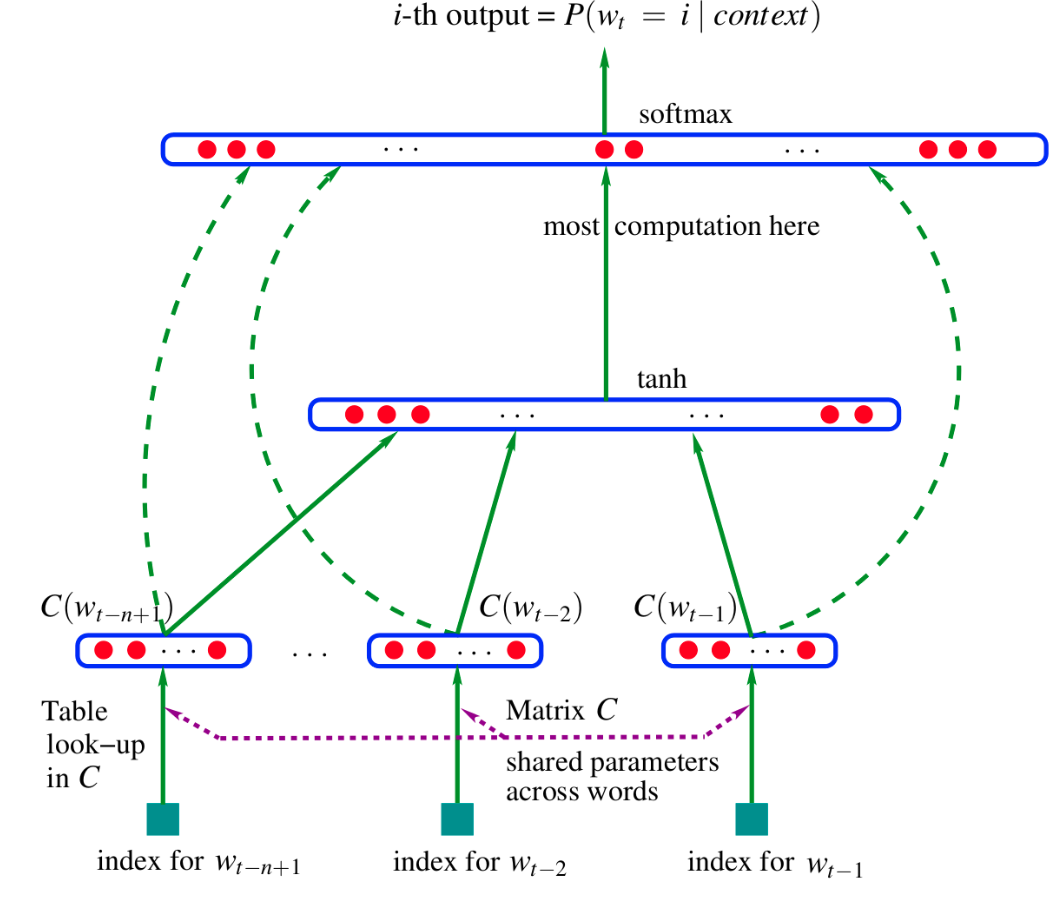
\includegraphics[width=0.8\textwidth]{figs/bengio_nn.png}
    \caption{Bengio's Neural Network Architecture for Neural Probabilistic Language Model}
    \label{fig:nn:bengio}
\end{figure}
For each input sequence, the neural network outputs a vector $y \in \mathbb{R}^{|V|}$, where $y_{i}$ is the unnormalized log-probability that the $t^{th}$ word in the sequence is $w_{i}$.
\begin{equation}
y = b + Wx + Utanh(d + Hx)
\end{equation}
where $tanh$ is the hyperbolic tangent applied to introduce non-linearity and $x$ is the word feature layer activation vector constructed by the concatenation of the context word vectors,
\begin{equation}
x = (C(w_{t-1}), C(w_{t-2}), \ldots, C(w_{t-n+1}))
\end{equation}
The unnormalized log probabilities in $y$ are converted to positive probabilities summing to $1$ by using a \emph{softmax} output layer that computes, 
\begin{equation}
P(w_{t} = i | w_{t-1}, \ldots, w_{t-n+1}) = \frac{e^{y_{w_t}}}{\sum_{i}e^{y_{i}}}
\end{equation}
The parameters of the model $(b, d, W, U, H)$ and the word vectors $C$ are estimated by maximizing the log-likelihood of the training corpus.

\subsection{Log-Linear Models}
\label{sec:word2vec}
Simple log-linear models are proposed in \cite{mikolov2013efficient} as opposed to the non-linear NPLM model to bring down the training time complexity without sacrificing with the quality of the word vectors. \todo{Also these models are based on the Distributional Hypothesis} The models bring down the complexity of learning vectors by not having a non-linear layer and matrix weighting of the input vectors that are the costliest operations in NPLM. The two models proposed in \cite{mikolov2013efficient} (word2vec) are Continuous Bag-of-Words and Continuous Skip-Gram model, described below.

\subsubsection{Continuous Bag-of-Words}
\label{sec:cbow}
The Continuous Bag-of-Words (CBOW) model is different from the NPLM in that the projection layer is shared for all words; i.e. all words get projected into the same hidden layer vector (their vectors are averaged). This architecture hence neglects the ordering of the words as opposed to NNLM that uses the concatenation of input vectors for the projection layer. The training criteria in this model is to to classify the current (middle) word given its context. It also uses word sequence from the future to aid this task with the relaxation that the aim is not to learn a language model. The model architecture is given in Figure~\ref{fig:nn:cbow}.
\begin{figure}[h!]
    \centering
        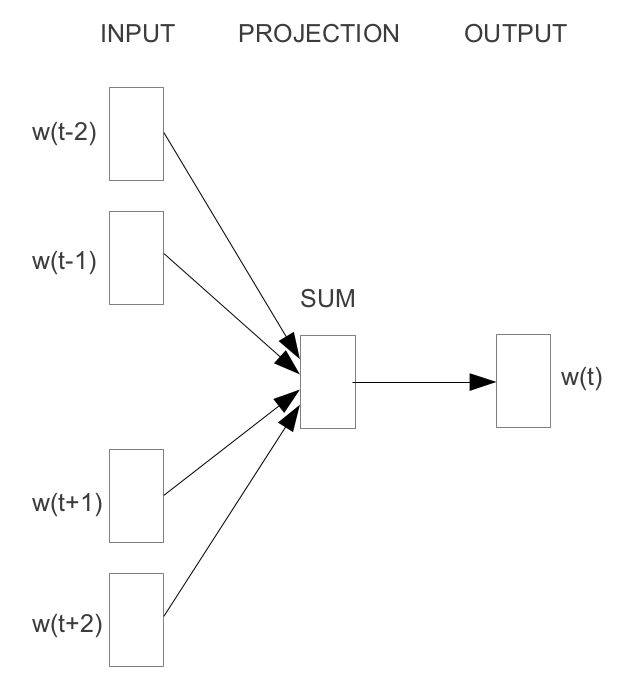
\includegraphics[width=0.5\textwidth]{figs/mikolov_cbow.png}
    \caption{Continuous Bag-of-Words Model (CBOW) \todo{Add ref?}}
    \label{fig:nn:cbow}
\end{figure}
The model first computes the hidden layer vector $h$, 
\begin{equation}
h(w_{t-k}, \ldots, w_{t+k}) = \frac{w_{t-k} + \ldots + w_{t-1} + w_{t+1} + \dots + w_{t+k}}{2k}
\end{equation}
where, $w_{t-i}$ is the $i$-th previous word in the context of the middle word $w_{t}$ and $k$ is the window length.
The neural network then computes a unnormalized log-probability vector $y$ similar to Sec.\ref{sec:bengio}, and uses the \emph{softmax}-classifier to estimate $P(w_{t}|w_{t-k}, \ldots, w_{t+k})$,
\begin{equation}
y = b + Uh(w_{t-k}, \ldots, w_{t+k})\\
\end{equation}
\begin{equation}
\label{eq:cbow:prob}
P(w_{t}|w_{t-k}, \ldots, w_{t+k}) = \frac{e^{y_{w_t}}}{\sum_{i} e^{y_{i}}}
\end{equation}
The parameters of the CBOW model, $(b, U)$ and the word vectors ($w_{i}$) are learned by maximizing the average log probability (Eq.~\ref{eq:cbow:prob}) of the training corpus.

\subsubsection{Continuous Skip-gram}
This model is similar to the CBOW model, but instead of predicting the middle word based on the context, it tries to maximize the classification of a word based on another word in the context. More precisely, given each word, the skip-gram model tries to predict words within a certain range before and after the current word. The model architecture is given in Figure~\ref{fig:nn:skip}
\begin{figure}[h!]
    \centering
        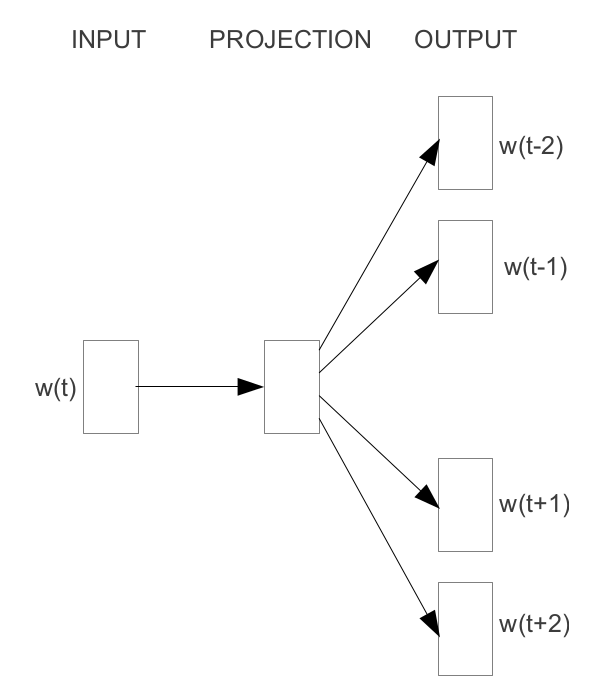
\includegraphics[width=0.4\textwidth]{figs/mikolov_skip.png}
    \caption{Continuous Skip-gram Model \todo{Add ref?}}
    \label{fig:nn:skip}
\end{figure}
Formally, given a sequence of words in a context $w_{t-k}, \ldots, w_{t+k}$, the skip-gram model defines $P(w_{t+j}|w_{t})$ using the \emph{softmax}-classifier in the following manner,
\begin{equation}
\label{eq:skip:prob}
P(w_{t+j}|w_{t}) = \frac{e^{(v_{w_{t}} \cdot v_{w_{t+j}} )} }{\sum_{i} e^{(v_{w_{t}} \cdot v_{w_{i}})} }
\end{equation}
The only parameters of the Skip-gram model are the word vectors ($v_{w_{i}}$) that are learned by maximizing the average log probability (Eq.~\ref{eq:skip:prob}) of predicting all the context words for all the words in the training corpus.

The CBOW and the Skip-gram models use the \emph{hierarchical softmax} \citep{morin2005hierarchical} instead of the full softmax to speed-up the learning process.

The quality of the word vectors is tested using the \emph{Semantic-Syntactic Word Relationship test} that evaluates the model performance on retrieving semantically and syntactically similar words to the given test words. The word vectors learned using the skip-gram model are also shown to encode many linguistic regularities and pattern \citep{mikolov2013linguistic} and show additive compositionality using simple vector arithmetics. For example, the result of the vector calculation $vec(Madrid) - vec(Spain) + vec(France)$ is closest to $vec(Paris)$ than any other word vectors.

\subsubsection{Dependency-based Word Embeddings}
Instead of using bag-of-words based context as used in \emph{NPLM} and \emph{word2vec}, \cite{levy2014dependencybased} use arbitrary contexts to investigate its effects on the word vectors and the properties they encode. The most important of their techniques is to derive the contexts based on the syntactic relations that the word participates is. For each word $w$ and its modifiers $m_1, \ldots, m_k$ found using the parse tree of the sentence, contexts $(m_{1}, lbl_{1}, \ldots, m_{k}, lbl_{k})$ are extracted, where $lbl$ is the type of the dependency relation between word and the modifier and $lbl^{-1}$ is used to mark the inverse-relation. An example of the contexts extracted for a sentence is given in Figure~\ref{fig:dep:context}.
\begin{figure}[h!]
    \centering
        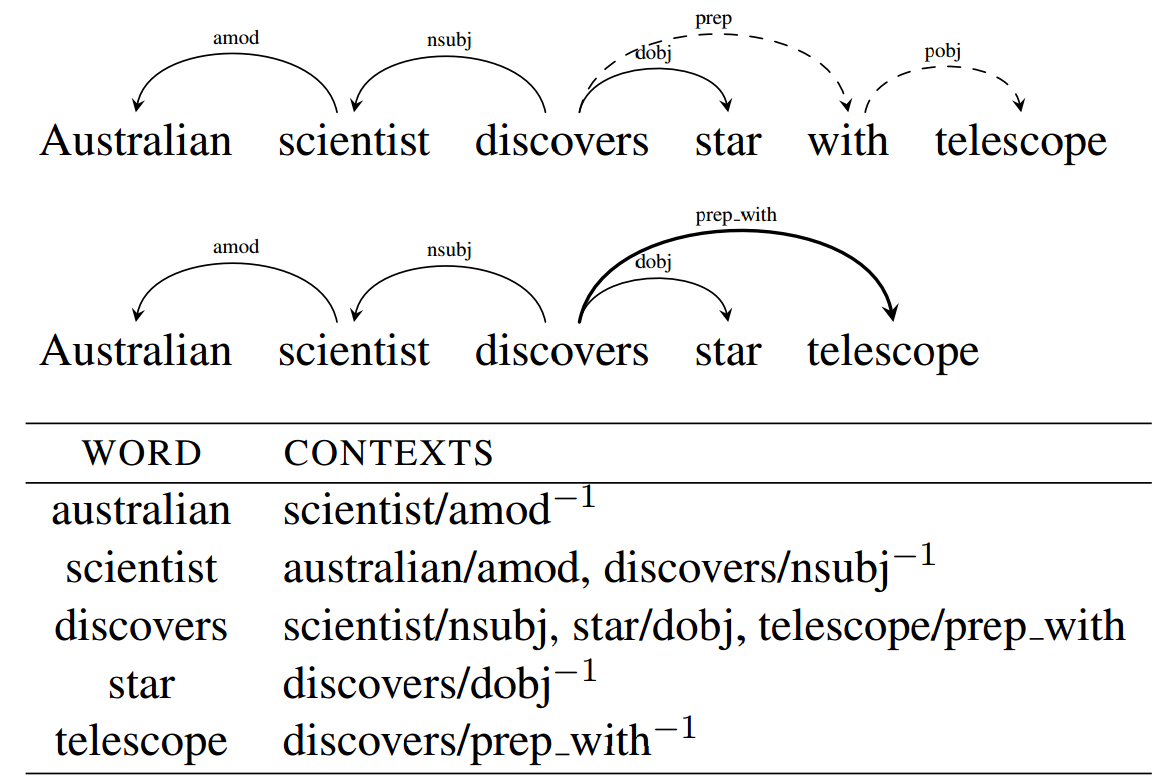
\includegraphics[width=0.7\textwidth]{figs/dependency_context.png}
    \caption{Dependency-based context extraction example \todo{Add ref?}}
    \label{fig:dep:context}
\end{figure}
After extracting the contexts, their model uses the neural network architecture and the training objective of the skip-gram model to learn word vectors. On comparison to the vectors learned from the skip-gram model on the tasks of \emph{topical similarity} and \emph{functional similarity} estimation, it is found that the vectors learned from this model perform better on the \emph{functional similarity} task that expects word vectors to encode syntactic relationships better. In the task of \emph{topical similarity} estimation, the vectors from the skip-gram model performed better as they encode semantic similarity between words because of the bag-of-words context used during training.

\section{Document Embeddings}
\label{sec:document_embeddings}
In the previous section we saw how distributed word embeddings that encode semantic similarity can be learned from text. 
Though these semantic word spaces are very useful for a lot of tasks, their ability to capture the complexity and compositionality of human language is limited. 
Word embeddings cannot be directly used to represent longer phrases, sentences and documents to express their meaning. 
Tasks such as word sense disambiguation, sentiment analysis, text categorization etc. all require the text representation to capture the semantic content of the text for better inputs to learning algorithms as compared to a simple bag-of-words model. 

Progress towards learning distributed representations for longer pieces of text, such as phrase-level or sentence-level representations [\cite{mitchell2010composition}, \cite{zanzotto2010estimating}, \cite{yessenalina2011compositional}, \cite{grefenstette2013multi}, \cite{mikolov2013distributed}] that capture semantic compositionality has been promising, but most models do not go beyond simple weighted average of word vectors to represent longer texts. 
\cite{socher2013recursive} proposes a more sophisticated approach using recursive tensor neural network where the dependency parse-tree of the sentence is used to compose word vectors in a bottom-up approach to represent sentences for sentiment classification of phrases and sentences. 
Both the techniques have weaknesses for learning document representations. The first approach is analogous to a bag-of-words approach and neglects word order while representing documents whereas the second approach considers syntactic dependencies but cannot go beyond sentences as it relies on parsing.

%\subsection{Learning Document Embeddings : Our Approach}
Below we present our model on learning universal distributed vector representations for documents and words in the corpus such that,
\begin{enumerate}
\item The learned vectors encode semantic and topical content of the documents and words.
\item Semantically similar documents/words have similar vector representations.
\end{enumerate}
%Our model is inspired by the work on continuous bag-of-words model \citep{mikolov2013efficient} and \citep{le2014distributed} model of learning representations for sentences and paragraphs. 
To learn vectors that satisfy $1.$ and $2.$ above, we hypothesize that document representations should be learned such that they can aid in the prediction of words in a given word sequence from the document. In the sections below we formally introduce the problem and present our model to learn document and word vector representations.

\subsection{Problem Setup}
Given a set of documents, $\setD=\{d_{1}, \ldots, d_{|\setD|}\}$ and a vocabulary of words, $\setW$ constructed using the set of documents, we wish to embed each document $d_{i} \in$ \setD and each word in the vocabulary onto the same $k$-dimensional space such that the learned vectors encode semantic content of the entities. 

For every sequence of words $w_{t-c}, \ldots, w_{t+c}$ in, say document $d_{i}$, we wish to estimate the probability $p(w_{t}|d_{i}, w_{t-c}, \ldots, w_{t-1}, w_{t+1}, \ldots, w_{t+c})$ of predicting the middle word in the sequence using the information about the document and the words in the context. 
We will estimate this probability using the vector representations for documents and words and learn vectors such that the probability of predicting the middle word in the context correctly is maximized.

\subsection{Our Model}
\label{sec:docem_ourmodel}
A document $d_{i} \in \setD$, indexed by `$i$', in our model is represented by a vector $\vecdi{i} \in \mathbb{R}^{k}$, which is also the $i$-th column of the matrix $\matD = \left[\vecdi{1}, \ldots, \vecdi{|\setD|}\right] \in \mathbb{R}^{k \times |\setD|}$. 
Similarly, a word indexed by `$i$' in the vocabulary $\setW$ is represented by vector $\vecwi{i} \in \mathbb{R}^{k}$, which is also the $i$-th column of the matrix $\matW = \left[\vecwi{1}, \ldots, \vecwi{|\setW|}\right] \in \mathbb{R}^{k \times |\setW|}$.

Given a sequence $(w_{t-c}, \ldots, w_{t+c})$ of $2c+1$ words and the document it occurs in, our training objective is to maximize the probability of correctly predicting the middle word $w_{t}$ using the surrounding context words $(w_{t-c}, \ldots, w_{t-1}, w_{t+1}, \ldots, w_{t+c})$, which we now denote as $context$ as a shorthand, and the information about the document in terms of their distributed vector representations. 
Therefore, our training objective is to maximize the probability $p(w_{t} | d_{i}, context)$ of correctly predicting the middle word using the information about the surrounding words and the document the sequence occurs in. 

To learn distributed word and document representations, we present a neural network model using which we,
\begin{enumerate}
\item Represent each word and document in the corpus by a $k$-dimensional distributed representation stored as vectors in the matrices $\matW$ and $\matD$, respectively.
\item Estimate the probability of predicting the middle word in a sequence, given the document it occurs in, using the vector representation of the document and the words in the context.
\item Learn the word and document vectors simultaneously with the parameters of the function to estimate the probability.
\end{enumerate}
The architecture for the proposed neural network is given in Fig.~\ref{fig:nn:archi}.
Also note that the word vector representations learned and stored in the matrix $\matW$ are universal representations and shared across all documents and contexts.
\begin{figure}[h!]
    \centering
        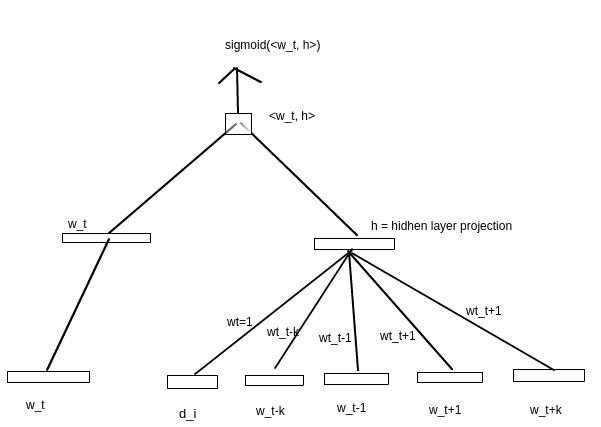
\includegraphics[width=0.9\textwidth]{figs/nn_arch.png}
    \caption{GloDETC : Neural Network Architecture \todo{Change figure}}
    \label{fig:nn:archi}
\end{figure}

%\para{Projection Layer (Context Representation)} : 
\subsubsection{Projection Layer (Context Representation)}
We represent the context(words surrounding the middle word to be predicted) and the document together in the same projection layer, denoted by $h_{c} \in \mathbb{R}^{k}$, by taking a weighted sum of the corresponding vector representations. 
The weights for the context words $\Lambda = \{\wgt{i} | i=\{t-c, \ldots, t-1, t+1, \ldots, t+c\}\}$ are kept universal for different sequences across the corpus as we expect the weights to learn some kind of syntactic quality of the language to better represent the context. Also the weight corresponding to the document vector is kept constant at $1$ as we expected the document to have equal contribution to all sequences. This also gave the best results.
We also (unsuccessfully) experimented by taking matrix weights instead of scalar weights($\wgt{i}$) to learn better syntactic qualities of the language. 

\begin{equation}
\label{eq:hidden_vec}
h_{c} = \vecdi{i} + \wgt{t-c}\vecwi{t-c} + \ldots + \wgt{t-1}\vecwi{t-1} + \wgt{t+1}\vecwi{t+1} + \wgt{t+c}\vecwi{t+c}
\end{equation}

%\textbf{Probability Prediction} : 
\subsubsection{Estimating Prediction Probability}
We expect in absence of any non-linearity that the projection layer vector should be aligned to the correct middle word of the sequence. Hence we estimate the probability of predicting the word $w_{t}$ as the middle word in the following manner. 
\begin{enumerate}
\item An output score $s_{w_{i}} \in \mathbb{R}$ for every $w_{i}$ in the vocabulary is estimated by,
\begin{equation}
\label{eq:nn_score}
s_{w_{i}} = \sigma(\vecwi{w_{i}}\cdot h_{c})
\end{equation}
where $\sigma(z) = \frac{1}{1+e^{-z}}$ is the standard sigmoid function. 
\item After calculating the score for each of the word in the vocabulary, we use the \emph{softmax} classifier to estimate the probability of predicting the actual correct word $w_{t}$ as the middle word in the sequence,
\begin{equation}
\label{eq:soft_prob}
p(w_{t} | d_{i}, w_{t-c}, \ldots, w_{t-1}, w_{t+1}, \ldots, w_{t+c}) = \frac{e^{s_{w_{t}}}}{\sum_{i \in \setW} e^{s_{i}}}
\end{equation}
\end{enumerate}

%\textbf{Training Objective} : 
\subsubsection{Training Objective}
The training data $\traindata$, is composed of $M$ training sequences each of which consists a $2c+1$ length sequence of words and the document index it belongs to. For example, $t = \{d^{(m)}_{i}, w^{(m)}_{t-c}, \ldots, w^{(m)}_{t+c}\}$ represents the $m^{th}$ training sequence in $\traindata$.  

Given the training data $\traindata$, our objective is to learn an optimum parameter set $\Theta = (\matD, \matW, \Lambda)$ consisting of the document and word vector matrices and the projection layer weights for the context words, by maximizing the average log probability of estimating the middle word correctly in all the training word sequences where the probability of estimating the middle word as $w_{i}$ is given by Eq.~\ref{eq:soft_prob}. Therefore, 
\begin{equation}
\label{eq:paramter_argmax}
\hat{\Theta} =  \argmax_{\Theta}~l(\traindata, \Theta)
\end{equation}
\begin{equation}
\label{eq:training_objective}
l(\traindata, \Theta) = \frac{1}{M}\sum_{m=1}^{M} \log \left[p(w^{(m)}_{t} | d^{(m)}_{i}, w^{(m)}_{t-c}, \ldots, w^{(m)}_{t-1}, w^{(m)}_{t+1}, \ldots, w^{(m)}_{t+c})\right]
\end{equation}
To learn the optimize the above training objective, we can use the Stochastic Gradient Descent(SGD) algorithm to find gradient of the objective function (Eq.~\ref{eq:training_objective}) w.r.t. to the individual parameters $\theta_{i}$ and apply the update rule as follows,
\begin{equation}
\label{eq:update_theta}
\theta^{(x)}_{i} = \theta^{(x-1)}_{i} + \gamma\frac{\partial l(\traindata, \Theta)}{\partial \theta_{i}}
\end{equation}
where $x$ is the current iteration number and $\gamma$ is the learning rate. Also note that we add the gradient to $\theta^{(x)}_{i}$ because we wish to maximize the training objective.
Updating the parameters for sufficient number of iterations should yield the optimum document and word vectors along with the weights for the neural network.

\subsubsection{Noise Contrastive Estimation}
As we see in Eq~\ref{eq:soft_prob}, estimating the probability for each training word sequence requires a sweep through the whole vocabulary of size $|\setW|$ which can be a very expensive computation given that typical vocabulary sizes range from a few tens to a few hundreds of thousand words for large datasets. Approaches to reduce this training time, such as, use of hierarchical soft-max \citep{morin2005hierarchical} and use of importance sampling to approximate the likelihood gradient \citep{bengio2003quick}, \citep{bengio2008adaptive} have been proposed. Using hierarchical softmax reduces the training time from linear to logarithmic in vocabulary size but is considerable more involved and finding well-performing trees is not trivial. Also, though importance sampling provides substantial speedups, it suffers from stability problems.

\textbf{Noise Contrastive Estimation (NCE)} \citep{gutmann2012noise} is method for fitting unnormalized probabilities by reducing the problem of \emph{density estimation} to \emph{probabilistic binary classification}. It has also been adapted to NPLM (Sec.~\ref{sec:bengio}) \citep{mnih2012fast} and learning word embeddings \cite{mnih2013learning} and shows significant improvements in training time with no considerable degradation in the quality of word vectors learned.

The basic idea of NCE is to train a logistic classifier to distinguish between the correct middle word in the given word sequence and corrupt samples from some ``noise'' distribution. Therefore, given a training sequence of the form $t = \{d^{(m)}_{i}, w^{(m)}_{t-c}, \ldots, w^{(m)}_{t+c}\}$, our training objective now is to train a classifier such that it can distinguish between positive training sample $w^{(m)}_{t}$ as positive example and negative training samples $w_{x}$ drawn from a noise distribution $P_{n}(w)$ as negative examples for the middle word given the surrounding words (context) and the document the sequence belongs to.

Our training data $\traindata$ is now converted to a set of labeled sequences of the form 
%$$t = \left[ \{d^{(m)}_{i}, w^{(m)}_{t-c}, \ldots, w^{(m)}_{t+c}\}, Y^{(m)}=1 \right]^{m=M}_{m=1}$ 
$ \{d^{(m)}_{i}, w^{(m)}_{t-c}, \ldots, w^{(m)}_{t+c}, Y^{(m)}=1\}^{m=M}_{m=1} $
where $Y=1$ denotes that the sequence is a positive sample occurring in the corpus. For every positive training sequence $t$ we also have $n$ corrupt training sequences where in each of them only the middle word $w_{t}$ has been replaced by a corrupt word sampled from the noise distribution $P_{n}(w)$ and the value of the label $Y=0$. Therefore, for every positive training example there exists $n$ negative training examples and the total number of training samples now in $\traindata$ is $M + nM$. We now need to train a binary classifier such that, given a sequence of words and the document it belongs to, it can predict correctly whether the sequence is legitimate (correct value of the label indicator $Y$). 

Given a training sequence we estimate the probability that the given sequence is positive using,
\begin{equation}
\label{eq:label1}
P(Y=1|d_{i}, w_{t-c}, \ldots, w_{t+c}, \Theta) = \sigma(\vecwi{w_{t}} \cdot h_{c})
\end{equation}
where $h_{c}$ is the projection layer vector calculated using Eq.~\ref{eq:hidden_vec}. Similarly, the probability of estimating that a given sequence is corrupt is given by,
\begin{equation}
\label{eq:label0}
P(Y=0|d_{i}, w_{t-c}, \ldots, w_{t+c}, \Theta) = 1 - \sigma(\vecwi{w_{t}} \cdot h_{c})
\end{equation}
From Eq.~\ref{eq:label1} and Eq.~\ref{eq:label0} we get,
%Therefore, the probability of $Y$ taking the value $0$ or $1$ is,
\begin{equation}
\label{eq:prob_y}
P(Y|d_{i}, w_{t-c}, \ldots, w_{t+c}, \Theta) = [\sigma(\vecwi{w_{t}} \cdot h_{c})]^{Y}[1 - \sigma(\vecwi{w_{t}} \cdot h_{c})]^{1-Y}
\end{equation}
As a shorthand notation, we would express the probability estimation in Eq.~\ref{eq:prob_y} as $P_{\Theta}(Y)$.

\subsubsection{New Training Objective}
Our new training objective involves maximizing the log-likelihood of observing the modified training data $\traindata$ that includes the negative examples sampled from the noise distribution $P_{n}(w)$ along with the original positive training sequences. 	
\begin{equation}
\label{eq:new_argmax}
\hat{\Theta} =  \argmax_{\Theta}~l(\traindata, \Theta)
\end{equation}
\begin{equation}
\label{eq:new_training_objective}
l(\traindata, \Theta) = \sum_{m=1}^{M + nM} \log P_{\Theta}(Y_{m} = Y^{(m)})
\end{equation}
where $Y_{m}$ is the predicted label for the $m$-th training sequence and,
\begin{equation}
\label{eq:log_P}
\log P_{\Theta}(Y_{m} = Y^{(m)}) = Y^{(m)}\log \sigma(\vecwi{w^{(m)}_{t}} \cdot h^{(m)}_{c}) + (1 - Y^{(m)})\log (1 - \sigma(\vecwi{w^{(m)}_{t}} \cdot h^{(m)}_{c}))
\end{equation}

\subsubsection{Parameter Estimation}
\label{sec:para_esti_doc}
To learn the optimum parameters $\Theta = (\matD, \matW, \Lambda)$ we would maximize the log-likelihood of observing the training data given in Eq~\ref{eq:new_argmax} using the Stochastic Gradient Descent(SGD) algorithm described below. 

Firstly, for the SGD algorithm we would need to calculate the gradient of the log probability estimate (Eq~\ref{eq:log_P}) with respect to individual parameters $\theta \in \Theta$. The derivative of the log probability estimate w.r.t. to a parameter $\theta \in \Theta$ is given by,
\begin{align}
\frac{\partial \log P_{\Theta}(Y_{m}=Y^{(m)})} {\partial \theta} &= \left[ Y^{(m)}\frac{1}{\sigma(d^{(m)})} - (1-Y^{(m)})\frac{1}{(1 - \sigma(d^{(m)}))}\right] \frac{\partial \sigma(d^{(m)})}{\partial \theta} \\
&= \left[ Y^{(m)}\frac{1}{ \sigma(d^{(m)})} - (1 - Y^{(m)})\frac{1}{(1 - \sigma(d^{(m)}))}\right] \left[\sigma(d^{(m)})(1-\sigma(d^{(m)}))\right]\frac{\partial d^{(m)}}{\partial \theta} \\
\frac{\partial \log P_{\Theta}(Y_{m}=Y^{(m)})} {\partial \theta} &= \left[ Y^{(m)} - \sigma(d^{(m)})\right] \frac{\partial d^{(m)}}{\partial \theta}
\end{align}
where $d^{(m)} = (\vecwi{w^{(m)}_{t}} \cdot h^{(m)}_{c})$ is the dot-product of the projection layer vector with the word vector for the middle word. Therefore,
\begin{equation}
\label{eq:partial_theta}
\frac{\partial \log P_{\Theta}(Y_{m}=Y^{(m)})} {\partial \theta} = \left[ Y^{(m)} - \sigma(\vecwi{w^{(m)}_{t}} \cdot h^{(m)}_{c})\right] \frac{\partial (\vecwi{w^{(m)}_{t}} \cdot h^{(m)}_{c})}{\partial \theta}
\end{equation}
For any training sequence $m$, there are four types of parameters $\theta$ that need to be updated. Firstly, the document vector for $d^{(m)}_{i}$, the middle word vector for word $w^{(m)}_{t}$, word vectors for context words $w^{(m)}_{t+j}$ and the neural network weights $\wgt{i}$. The derivate $\frac{\partial (\vecwi{w^{(m)}_{t}} \cdot h^{(m)}_{c})}{\partial \theta}$ w.r.t. each of them is given by,
\begin{equation}
\label{eq:partial_doc}
\frac{\partial (\vecwi{w^{(m)}_{t}} \cdot h^{(m)}_{c})}{\partial \vecdi{d^{(m)}_{i}}} = \vecwi{w^{(m)}_{t}}
\end{equation}
\begin{equation}
\label{eq:partial_w_t}
\frac{\partial (\vecwi{w^{(m)}_{t}} \cdot h^{(m)}_{c})}{\partial \vecwi{w^{(m)}_{t}}} = h^{(m)}_{c}
\end{equation}
\begin{equation}
\label{eq:partial_w_t-k}
\frac{\partial (\vecwi{w^{(m)}_{t}} \cdot h^{(m)}_{c})}{\partial \vecwi{w^{(m)}_{t+j}}} = \wgt{t+j}* \vecwi{w^{(m)}_{t}}
\end{equation}
\begin{equation}
\label{eq:partial_wgt_t-k}
\frac{\partial (\vecwi{w^{(m)}_{t}} \cdot h^{(m)}_{c})}{\partial \wgt{t+j}} = \vecwi{w^{(m)}_{t}} \cdot \vecwi{w^{(m)}_{t+j}}
\end{equation}

Therefore the derivative of the log-probability estimate w.r.t. the 
\begin{enumerate}
\item
\textbf{Document Vector} : 
\begin{equation}
\label{eq:grad_doc}
\frac{\partial \log P_{\Theta}(Y_{m}=Y^{(m)})} {\partial \vecdi{d^{(m)}_{i}}} = \left[ Y^{(m)} - \sigma(\vecwi{w^{(m)}_{t}} \cdot h^{(m)}_{c})\right] \vecwi{w^{(m)}_{t}}
\end{equation}
\item 
\textbf{Middle Word} : 
\begin{equation}
\label{eq:grad_mword}
\frac{\partial \log P_{\Theta}(Y_{m}=Y^{(m)})} {\partial \vecwi{w^{(m)}_{t}}} = \left[ Y^{(m)} - \sigma(\vecwi{w^{(m)}_{t}} \cdot h^{(m)}_{c})\right] h^{(m)}_{c}
\end{equation}
\item 
\textbf{Context Word} : 
\begin{equation}
\label{eq:grad_cword}
\frac{\partial \log P_{\Theta}(Y_{m}=Y^{(m)})} {\partial \vecwi{w^{(m)}_{t+j}}} = \left[ Y^{(m)} - \sigma(\vecwi{w^{(m)}_{t}} \cdot h^{(m)}_{c})\right] \wgt{t+j} \vecwi{w^{(m)}_{t}}
\end{equation}
\item 
\textbf{Neural Network Weight} : 
\begin{equation}
\label{eq:grad_wgt}
\frac{\partial \log P_{\Theta}(Y_{m}=Y^{(m)})} {\partial \wgt{t+j}} = \left[ Y^{(m)} - \sigma(\vecwi{w^{(m)}_{t}} \cdot h^{(m)}_{c})\right] (\vecwi{w^{(m)}_{t}} \cdot \vecwi{w^{(m)}_{t+j}})
\end{equation}
\end{enumerate}
According to the SGD algorithm, the update to be made to a parameter $\theta \in \Theta$ on observing a training sequence $m$ is therefore given in Eq.~\ref{eq:update_reg}. We also include $L_{2}$ regularization for the parameters as it helps in avoiding overfitting and restricts the  parameters to  blow up in value.
\begin{equation}
\label{eq:update_reg}
\theta^{(i+1)} \leftarrow \theta^{(i)} + \gamma \left[\frac{\partial \log P_{\Theta}(Y_{m} = Y^{(m)})}{\partial \theta^{(i)}} - \beta \theta^{(i)} \right]
\end{equation}
here $\theta^{(i)}$ denotes the value of the parameter in the $i$-th iteration, $\theta^{i+1}$ is the value after the update, $\gamma$ is the learning rate and $\beta$ is the regularization constant.
The update rules for the document vector, word vectors and the neural network weights are hence given by,
\begin{enumerate}
\item 
\textbf{Document Vector} : 
\begin{equation}
\label{eq:update_doc}
(\vecdi{d^{(m)}_{i}})^{(i+1)} = (\vecdi{d^{(m)}_{i}})^{(i)} + \gamma \left[ (Y^{(m)} - \sigma(\vecwi{w^{(m)}_{t}} \cdot h^{(m)}_{c}))\vecwi{w^{(m)}_{t}} - \beta\vecdi{d^{(m)}_{i}} \right]
\end{equation}
\item 
\textbf{Middle Word Vector} : 
\begin{equation}
\label{eq:update_mword}
(\vecwi{w^{(m)}_{t}})^{(i+1)} = (\vecwi{w^{(m)}_{t}})^{(i)} + \gamma \left[ (Y^{(m)} - \sigma(\vecwi{w^{(m)}_{t}} \cdot h^{(m)}_{c})) h^{(m)}_{c} - \beta\vecwi{w^{(m)}_{t}} \right]
\end{equation}
\item 
\textbf{Context Word Vectors} : 
\begin{equation}
\label{eq:update_cword}
(\vecwi{w^{(m)}_{t+j}})^{(i+1)} = (\vecwi{w^{(m)}_{t+j}})^{(i)} + \gamma \left[(Y^{(m)} - \sigma(\vecwi{w^{(m)}_{t}} \cdot h^{(m)}_{c}))\wgt{t+j} \vecwi{w^{(m)}_{t}} - \beta\vecwi{w^{(m)}_{t+j}} \right]
\end{equation}
\item 
\textbf{Neural Network Weights} : 
\begin{equation}
\label{eq:update_wgt}
\wgt{t+j}^{(i+1)} = \wgt{t+j}^{(i)} + \gamma \left[ (Y^{(m)} - \sigma(\vecwi{w^{(m)}_{t}} \cdot h^{(m)}_{c}))(\vecwi{w^{(m)}_{t}} \cdot \vecwi{w^{(m)}_{t+j}}) -\beta\wgt{t+j} \right]
\end{equation}
\end{enumerate}
To learn the vectors $\matD$, $\matW$ and weights $\Lambda$ we initialize them to small random vectors and scalars respectively and using Eqs.~\ref{eq:update_doc}, ~\ref{eq:update_mword}, ~\ref{eq:update_cword} and ~\ref{eq:update_wgt} we iterate through the training data, making the appropriate updates for a fixed number of epochs that is learned using the development data. For each training sequence we make one update to the document vector, $2c$ updates for the word vectors in the sequence and the neural network weights, where $c$ is the window length we consider while training. The complete algorithm for learning document and word vectors using our model is described in Algorithm~\ref{alg:doc_embeddings}.

\begin{algorithm}[h]
\begin{algorithmic}[1]
 \State \textbf{Input: } $\setD$, $k$, $c$, $n$, $\beta$, $\gamma$, $epochs$
 \State \textbf{Output: } Document Vectors $\matD$, Word Vectors $\matW$ 
 \State Extract Vocabulary $\setW$ from $\setD$
 \State $\setW \gets Extractfrom(\setD)$ 
 \State $\matD \gets random(\mathbb{R}^{k \times |\setD|})$
 \State $\matW \gets random(\mathbb{R}^{k \times |\setW|})$
 \State $\traindata \gets Extract from (\setD, c, n)$ \Comment{$|\traindata| = M + nM$}
 \State $\Lambda \gets \mathbf{1}^{2c}$ \Comment{$2c$-sized vector of 1s}
 \While{$epochs \geq 1$}
 \ForAll{$\{d_{i}, w_{t-c}, \ldots, w_{t+c}, Y\} \in \traindata$}
  \State $h_{c} \gets \vecdi{d_{i}} + \wgt{t-c}\vecwi{w_{t-c}} + \ldots + \wgt{t+c}\vecwi{w_{t+c}}$
  \State $\vecdi{d_{i}} \gets \vecdi{d_{i}} + \gamma \left[ (Y - \sigma(\vecwi{w_{t}} \cdot h_{c}))\vecwi{w_{t}} - \beta\vecdi{d_{i}} \right]$
  \State $\vecwi{w_{t}} \gets \vecwi{w_{t}} + \gamma \left[ (Y - \sigma(\vecwi{w_{t}} \cdot h_{c})) h_{c} - \beta\vecwi{w_{t}} \right]$
  \State $\vecwi{w_{t+j}} \gets \vecwi{w_{t+j}} + \gamma \left[(Y - \sigma(\vecwi{w_{t}} \cdot h_{c}))\wgt{t+j} \vecwi{w_{t}} - \beta\vecwi{w_{t+j}} \right]$
  \State $\wgt{t+j} \gets \wgt{t+j} + \gamma \left[ (Y - \sigma(\vecwi{w_{t}} \cdot h_{c}))(\vecwi{w_{t}} \cdot \vecwi{w_{t+j}}) -\beta\wgt{t+j} \right]$
  \State $epochs \gets epochs - 1$
  %compute(\vecdi{d_{i}}, \vecwi{w_{t-c}}, \ldots, \vecwi{w_{t-1}}, \vecwi{w_{t+1}}, \vecwi{w_{t+c}})$
 \EndFor 
 \EndWhile
 \\
 \Return $\matD, \matW$
\end{algorithmic}
\caption{Learning Document and Word Representations}
\label{alg:doc_embeddings}
\end{algorithm}

\subsubsection{Hyper-parameters}
\label{sec:hp_doc}
Our model, like any other, has hyper-parameters that need to be tuned for optimum model performance and learning high quality document and word vectors and the model parameters for achieving the the best accuracies in the task. Below we describe the hyper-parameters in our model and the effect they have on learning document representations.
\begin{enumerate}
\item \textbf{Embedding Dimensionality ($k$)} : The most important hyper-parameter in our model is the size of the document and word embedding vectors $k$. The embedding dimensionality needs to be big enough such that the document vectors can encode the different semantic topics across the corpus but shouldn't be very large so that it introduces noise in the vectors.

\item \textbf{Window  Size ($c$)} : The length of the sequence or the window size $c$, that we consider as context surrounding a word plays an important role in the vectors that are learned. While a smaller window could result in the negligence of important/similar words that surround the middle word, a large window could introduce noise in the context that can deteriorate the performance of the model.

\item \textbf{Number of Negative Samples ($n$)} : In NCE, the number of negative samples introduced in the training data per positive example plays an important role in deciding the trade-off between learning better word density distribution with larger $n$ while smaller $n$ leads to lesser training times. Hence, the number of negative samples introduced needs to be tuned using the development data.

\item \textbf{Number of Epochs} : The number of times we need to loop through the training data to learn the vectors needs to be optimized to prevent overfitting with large epochs while at the same time learn high quality representations.

\item \textbf{Learning Rate ($\gamma$)} : The learning rate used in the SGD algorithm plays an important role whose optimum value is dependent on the dataset and the objective function. While a smaller learning rate could harm the training time and convergence, a larger learning rate may lead to a case of non-convergence and poor parameters

\item \textbf{Regularization Constant ($\beta$)} : Regularization is introduced in the training objective to avoid overfitting of parameters by reducing model complexity. While a small value may not penalize complexity by enough, larger constants may inhibit the growing of parameters with a negative effect which required careful selection of the regularization constant dependent on the dataset.
\end{enumerate}
We explain the manner in which we tune these hyper-parameters later in Sec.~\ref{sec:exp_setup}.





	\chapter{Multi-Label Text Categorization}
\label{chapter:mltextcat}
In this chapter we will give an overview of the training data required for the document categorization task and present the multinomial logistic regression algorithm in context of the multi-label text categorization, discuss its advantages and similarity to matrix factorization and relational learning.

\section{Logistic Regression for Multi-label Document Categorization}
\label{sec:lrtc}
Introduced by \citep{hosmer1989applied}, Logistic Regression (LR) is a probabilistic binary classification regression model that, given labeled binary data, performs regression over the data and learns weight vectors to predict whether a given data point belongs to the positive or the negative class. 
The probability of the data point to belong in a class is estimated using the \emph{logistic (sigmoid) function}, hence the name logistic regression.

Logistic Regression, though is a technique to discriminate between two categories can be easily extended to classification between multiple categories which is then referred to as Multinomial Logistic Regression. 
Though we use use multinomial logistic regression for our task of multi-label text classification, for the sake of brevity we would refer to our algorithm as logistic regression.\

In the sections below we describe the training data required for the task of multi-label document classification, the logistic regression model as modified for the task and also its similarity to relational learning.

\subsection{Training Data}
\label{sec:trdata_lr}
The training data $\traindata$ is composed of a set of documents $\setD$, set of categories $\setC$ and data about in what categories do each of the documents belong to. 

\textbf{Document-Category Data} : 
Each document $d_{i}$ in $\setD$ belongs to atleast one category from $\setC$. To store this relational data between the documents and the categories, we create a database $\db$ in which for the $m$-th training instance we store tuple of the form $\{ d^{(m)}_{i}, c^{(m)}_{j}, y^{(m)}\}^{m=T}_{m=1}$ where $y^{(m)} \in \{0, 1\}$ denotes whether the document $d^{(m)}_{i}$ belongs the category $c^{(m)}_{j}$ or not. 

Mostly the data about document categories is given such that it is known what categories do the documents belong to, without conclusive information about whether a document necessarily does not belong to a particular category. In such cases, if we assume the given data to be complete, then along with positive data examples of the form, $\{ d_{i}, c_{j}, 1\}$, we introduce negative samples, $\{ d_{i}, c_{k}, 0\}$ for every category $c_{k}$ each document $d_{i}$ does not belong to. 
If the document-category data is viewed as a matrix with documents as rows and categories as columns, then in such case, we would only observe positive examples ($1$) in matrix but at sparse locations. To make the training data complete in such cases, we would fill the matrix with negative examples ($0$) at every empty location.

\textbf{Document Representations} : 
Along with the document-category data, the training data also composes of the document representations in the form of either bag-of-words representations or distributed document embeddings as learnt in Sec.~\ref{sec:document_embeddings}.  Therefore for every document $d_{i} \in \setD$ indexed by $i$, we have a vector representation $\vecdi{i} \in \mathbb{R}^{k}$ of the document.

%\subsection{Multi-label Document Categorization using LR}
\subsection{Logistic Regression Model}
For multi-label document categorization we extend the standard logistic regression (which is a binary classification algorithm) to,
\begin{enumerate}
\item Train from multi-labeled document-category data data 
\item Given a document-category pair $\{d_{i}, c_{j}\}$, estimate the probability of the document $d_{i}$ belonging to the category $c_{j}$.
\end{enumerate}
As we explained in Sec.~\ref{sec:document_embeddings}, we learn low-rank distributed vector representation for every document in the corpus. Similarly, for multi-label logistic regression, we represent each category $c_{i} \in \setC$ using a low-rank embedding $\vecci{c_{i}} \in \mathbb{R}^{k}$ of the same dimensionality as the document embeddings, $k$. Similar to $\matD$, we stack these category embeddings as columns in the matrix $\matC \in \mathbb{R}^{k \times |\setC|}$.

Given a document-category tuple of the form $\{d_{i}, c_{j}\}$, we estimate the probability of the document belonging to the category ($y = 1$) using the logistic function as,
\begin{equation}
\label{eq:prob_dc}
P(y=1|d_{i}, c_{j}, \matD, \matC) = \sigma(\vecdi{d_{i}}\cdot \vecci{c_{j}})
\end{equation}
This model is similar to the standard logistic regression (LR) as in standard LR for binary classification, we learn a universal weight vector $\mathbf{w}$ that is used to estimate the probability in Eq.~\ref{eq:prob_dc} instead of $\vecci{c_{j}}$. Here, because we have multiple categories, we learn multiple weight vectors (category embeddings) for each category separately and hence perform multiple binary classifications.

\subsubsection{Training Objective}
\label{sec:tro_lr}
As explained in Sec.~\ref{sec:trdata_lr}, the training data $\traindata$, is composed of $T$ tuples of the form $\{ d^{(m)}_{i}, c^{(m)}_{j}, y^{(m)}\}$. Our training objective involves learning optimum category embeddings such that for any unobserved document $d_{x} \notin \setD$, we should be able to predict the categories it belongs to.

For the $m$-th training instance $\{ d^{(m)}_{i}, c^{(m)}_{j}, y^{(m)}\}$, we denote the prediction that whether the document $d^{(m)}_{i}$ belongs the category $c^{(m)}_{j}$ by $y_{m}$. Therefore, if we estimate $d^{(m)}_{i}$ belongs $c^{(m)}_{j}$, $y_{m} = 1$ otherwise $y_{m} = 0$. Using Eq.~\ref{eq:prob_dc},
\begin{equation}
\label{eq:prob_trm}
P(y_{m}=1|d^{(m)}_{i}, c^{(m)}_{j}, \matD, \matC) = \sigma(\vecdi{d^{(m)}_{i}}\cdot \vecci{c^{(m)}_{j}})
\end{equation}
We denote the above probability estimate as $P_{\matD, \matC}(y_{m} = 1)$ for brevity. Therefore,
\begin{equation}
\label{eq:prob_trm_neg}
P_{\matD, \matC}(y_{m} = 0) = 1 - \sigma(\vecdi{d^{(m)}_{i}}\cdot \vecci{c^{(m)}_{j}})
\end{equation}
\begin{equation}
\label{eq:prob_bernouli}
P_{\matD, \matC}(y_{m}) = \sigma(\vecdi{d^{(m)}_{i}}\cdot \vecci{c^{(m)}_{j}})^{y_{m}}(1 - \sigma(\vecdi{d^{(m)}_{i}}\cdot \vecci{c^{(m)}_{j}}))^{1-y_{m}}
\end{equation}
To learn the optimum parameter set $\Theta = (\matC)$ consisting of the set of category embeddings, we would maximize the log-likelihood of observing the training data,
\begin{equation}
\label{eq:cembed_argmax}
\hat{\Theta} =  \argmax_{\Theta}~l(\traindata, \Theta)
\end{equation}\begin{equation}
\label{eq:new_to_lr}
l(\traindata, \Theta) = \sum_{m=1}^{T} \log P_{\matD, \matC}(y_{m} = y^{(m)})
\end{equation}
where,
\begin{equation}
\label{eq:log_P_lr}
\log P_{\matD, \matC}(y_{m} = y^{(m)}) = y^{(m)}\log \sigma(\vecdi{d^{(m)}_{i}}\cdot \vecci{c^{(m)}_{j}}) + (1 - y^{(m)})\log (1 - \sigma(\vecdi{d^{(m)}_{i}}\cdot \vecci{c^{(m)}_{j}}))
\end{equation}

\subsubsection{Parameter Estimation}
To learn the optimum parameters $\Theta=(\matC)$ we would maximize the log-likelihood of observing the training data given in Eq~\ref{eq:new_to_lr} using the Stochastic Gradient Descent(SGD) algorithm as described earlier in Sec~\ref{sec:para_esti_doc}. We first need to calculate the gradient of the log probability estimate (Eq.~\ref{eq:log_P_lr}) with respect to the category embeddings which is given by,
\begin{align}
\frac{\partial \log P_{\matD, \matC}(y_{m}=y^{(m)})} {\partial \vecci{c^{(m)}_{j}}} &= \left[ y^{(m)}\frac{1}{\sigma(s^{(m)})} - (1-y^{(m)})\frac{1}{(1 - \sigma(s^{(m)}))}\right] \frac{\partial \sigma(s^{(m)})}{\partial \vecci{c^{(m)}_{j}}} \\
&= \left[ y^{(m)}\frac{1}{\sigma(s^{(m)})} - (1-y^{(m)})\frac{1}{(1 - \sigma(s^{(m)}))}\right] \left[\sigma(s^{(m)})(1-\sigma(s^{(m)}))\right]\frac{\partial s^{(m)}}{\partial \vecci{c^{(m)}_{j}}} \\
\frac{\partial \log P_{\matD, \matC}(y_{m}=y^{(m)})} {\partial \vecci{c^{(m)}_{j}}} &= \left[ y^{(m)} - \sigma(s^{(m)})\right] \frac{\partial s^{(m)}}{\partial \vecci{c^{(m)}_{j}}}
\end{align}
where, $s^{(m)} = (\vecdi{d^{(m)}_{i}}\cdot \vecci{c^{(m)}_{j}})$ is the \emph{pre-sigmoid activation}. Therefore,
\begin{equation}
\frac{\partial \log P_{\matD, \matC}(y_{m}=y^{(m)})} {\partial \vecci{c^{(m)}_{j}}} = \left[ y^{(m)} - \sigma(\vecdi{d^{(m)}_{i}}\cdot \vecci{c^{(m)}_{j}})\right] \frac{\partial (\vecdi{d^{(m)}_{i}}\cdot \vecci{c^{(m)}_{j}})}{\partial \vecci{c^{(m)}_{j}}}
\end{equation}
\begin{equation}
\label{eq:grad_c}
\frac{\partial \log P_{\matD, \matC}(y_{m}=y^{(m)})} {\partial \vecci{c^{(m)}_{j}}} = \left[ y^{(m)} - \sigma(\vecdi{d^{(m)}_{i}}\cdot \vecci{c^{(m)}_{j}})\right] \vecdi{d^{(m)}_{i}}
\end{equation}
According to the SGD algorithm and Eq.~\ref{eq:update_reg}, the update to be made to the category embedding on observing the $m$-th training instance is given by Eq.~\ref{eq:update_cat}. We also include L2
regularization for the category embeddings as it helps in avoiding overfitting and restricts the embeddings to blow up in value.
\begin{equation}
\label{eq:update_cat}
(\vecci{c^{(m)}_{j}})^{(i+1)} = (\vecci{c^{(m)}_{j}})^{(i)} + \gamma \left[ ( y^{(m)} - \sigma(\vecdi{d^{(m)}_{i}}\cdot (\vecci{c^{(m)}_{j}})^{(i)}) \vecdi{d^{(m)}_{i}} -\beta(\vecci{c^{(m)}_{j}})^{(i)} \right]
\end{equation}
Here $(\vecci{c^{(m)}_{j}})^{(i)}$ and $(\vecci{c^{(m)}_{j}})^{(i+1)}$ are the category embeddings before and after the update, respectively, $\gamma$ is the learning rate of the algorithm and $\beta$ is the regularization constant used for the $L_{2}$ regularization. 

As explained in Sec.~\ref{sec:para_esti_doc}, we initialize the category embeddings $\matC$ to small random vectors and loop through the training data $\traindata$ until we reach convergence based on the development data. The complete algorithm for employing the logistic regression model for multi-label document categorization is given in Algorithm.\todo{Add algo}.

\section{Similarity to Relational Learning}
\label{sec:lr_similar_rl}
The multi-label document categorization can be viewed as a relational learning problem where the task is to find missing links between documents and categories or for new documents find what categories does it link to. Relational learning has a novel solution in Matrix Factorization which assumes that the relational data matrix has a low-rank structure and tries to factorize it as a product of two matrices representing the row and column entity factors. 

Therefore, if $R$ denotes the binary relational matrix, where rows and columns correspond to the entities of two different type and the entries $r(i, j) \in \{0,1\}$ of the matrix denotes the presence/absence of link between the $i$-th row and the $j$-th column entity. Employing matrix factorization would try to decompose the matrix $R$ into row and column factors, say $U$ and $V$ such that,
\begin{equation}
\label{eq:mf_decompose}
R = UV^{T}
\end{equation}
where, if $R \in \mathbb{R}^{m \times n}$ then $U \in \mathbb{R}^{m \times k}$ and $V \in \mathbb{R}^{n \times k}$, where $k < min(m, n)$ is the approximate rank of $R$. The rows of the matrix $U$ and $V$ store the factors/embeddings for the entities. As we see, such an approach tries to learn low-rank embeddings for the row and column entities and projects them on to the same $k$-dimensional space.

In our model of logistic regression for multi-label document classification, though we take a similar approach and learn category embeddings to project the categories along with the documents to the same $k$-dimensional space, our method has the following differences,
\begin{enumerate}
\item Instead of factorizing the document-category data matrix, $R$ using a linear matrix factorization approach as in Eq.~\ref{eq:mf_decompose}, we take a probabilistic approach and think of $R$ has a probabilistic database and estimate the probability of a document belonging to a particular category.

\item As we already learn document embeddings $\matD$ using our model described in Sec.~\ref{sec:docem_ourmodel}, we only learn the category embeddings matrix $\matC$ instead of learning embeddings for both kind of entities as done in Eq.~\ref{eq:mf_decompose} by learning both $U$ and $V$.
\end{enumerate}

\section{Advantages of Logistic Regression Learning Algorithm}
As shown above, we use a modified version of the Logistic Regression for multi-label document categorization that learns multiple classifiers (in terms of the category embeddings) for multi-labeling task. Even though learning algorithms that learn multiple independent classifiers have drawbacks as elucidated in Sec~\ref{sec:rw_multiple_classifiers}, our logistic regression style algorithm has a lot of advantages that make it a good choice for the document categorization task. Below we list some of the major advantages of the algorithm. 
\begin{enumerate}
\item 
Since we learn distributed embeddings for the categories in the same $k$-dimensional space as the documents and words it enables us to estimate the similarity within entities and between unrelated entities. It is as simple as taking a dot-product of the corresponding embeddings. For example, we can estimate the similarity between two or more categories or between categories and words that wouldn't be possible if some other learning technique was used. 

\item 
The major drawback of algorithms that learn multiple independent classifiers is their inability to capture and exploit the correlations among categories from the training data. As we exploit the low-rank structure of the document-category relational matrix by learning factors for categories we are able to learn correlations among categories in a way similar to as done by collaborative filtering.

\item 
Generally, document-category data is accompanied by additional relational data about documents and/or categories which is often incomplete. As has been shown in \cite{gupta2015collectively}, joint modeling of relations and entities using collective matrix factorization of multiple relational matrices can provide signification improvements in the relation prediction task. 
Our model, based on matrix factorization as shown in Sec~\ref{sec:lr_similar_rl}, can easily be extended to incorporate additional relational data and aid in improved database completion. 

\item \todo{Find missing categories??}
\end{enumerate}
	\chapter{Performance Evaluation}
\label{chapter:evaluations}
In this chapter we first introduce the datasets that we use for evaluating the efficacy of our document representations for the document categorization task. We then explain the details of our experimentatal setup and the different document representation techniques that form strong reference baselines for comparison. Then in the following sections we present the categorization results for  new documents and also results for imputing missing categories for documents that already have prior category information. 

\section{Datasets}
We perform our experimentation on 5 datasets that contain rich data about documents belonging to multiple categories simultaneously. One of the 5 datasets we use is the widely used Reuters-21578 collection, which is often considered a benchmark for evaluating text classification. The Reuters data set is richly multi-label and moderately-sized and has been used as a benchmark for many years which gives us the opportunity to compare our accuracy with previous state-of-art results. The other 4 datasets that we use for evaluation are, exclusive subsets of documents extracted from Wikipedia.


\subsection{Reuters-21578}
Reuters-21578 collection consists of documents published on the Reuters newswire in 1987. As the name suggests it has a total of 21758 documents assigned category labels from a set of 135 categories. Though most of the documents in the collection are multi-labeled, many documents are assigned only a single category. The Reuters-21578 dataset has over the years become a standard dataset for evaluating many information retrieval algorithms due to the the multi-label
nature of the collection and the large number of categories present in the collection that are overlapping and non-exhaustive. Relationships between the categories also makes it an interesting dataset to evaluate on, as the algorithms that capture the correlations between the categories are bound to perform better. Even though the dataset contains a reasonable number of documents and categories, it is very sparse making learning difficult.

Though there exist many processed versions of the collection, the \emph{ModApte} (Modified Apte) version is the most widely used version of the Reuters-21578 for evaluating multi-label classification algorithms. The \emph{ModApte} version predefines a train/test split by considering all documents published after a specific date for testing purposes and the rest for training. After the split the only categories considered are the ones that have at least one document in the training and test set. The number of documents, categories, words and other statistics of the Reuters(\emph{ModApte}) dataset are given in Table~\ref{reuter:data:stat}.

\begin{table}[h!]
%\tabcolsep=0.05cm
%\footnotesize
\begin{center}
\begin{tabular}{l c c c c c} % ccc ccc}
\toprule
& \textbf{$|\setD|$} & \textbf{$|\setC|$} & \textbf{$|\setW|$} & \textbf{Data Points} & \textbf{Sparsity}\\
\midrule
\textbf{Train Set}	& 7,767 & 90 & 39,853 & 9,585 & 0.0137 \\
\textbf{Test Set}	& 3,019 & 90 & 39,853 & 3,745 & 0.0138 \\
\bottomrule         
\end{tabular}
\caption{\label{reuter:data:stat}Statistics of the Reuters-21578 (\emph{ModApte}) Dataset}
\end{center}
\end{table}

\subsection{Wikipedia Datasets}
Wikipedia\footnote{www.wikipedia.org} is an open-access, free content Internet encyclopedia that contains articles about virtually everything. Along with the very large number of articles, Wikipedia also has a hierarchical cyclic \emph{Wikipedia Category Graph} that is used to label articles with the category labels relevant to them. 
Though the category graph is connected, it has a few major top-level categories within which all subsequent categories fall. For e.g. some of the top-level categories are \emph{Culture and Arts}, \emph{Geography}, \emph{Health}, \emph{History}, \emph{Mathematics}, \emph{Natural and Physical Sciences}, \emph{Philosophy} etc. Each of the top-level categories are further divided into deep trees of fine-grained categories that are assigned to the articles. 

The categories that are assigned to an article thus range from broader categories to fine-grained ones that are very difficult to assign via an automated system. For e.g. some of the categories assigned to an article on the musician \emph{Jimi Hendrix} are \emph{1942 Births}, \emph{1970 deaths}, \emph{American Rock Guitarists}, \emph{Musicians from Seattle}, \emph{Military Brats}, \emph{Alcohol-related deaths in England}. Automatic categorization of such granularity requires the document representation to capture the different semantic topics in the document with great accuracy.

To test the efficacy of our model on such a diverse, recent and real-life dataset, we extracted documents from 4 top-level categories in Wikipedia, namely \emph{Physics}, \emph{Biology}, \emph{Mathematics} and \emph{Sports}, in the following manner. For each of top-level category we compiled a list of all its child categories till a 3-level depth. To create the document-category dataset, we considered all the documents and the assigned categories that belonged to the compiled category list. The number of documents, categories, words and other statistics of the extracted datasets are given in Table~\ref{wiki:data:stat}.

\begin{table}[h!]
%\tabcolsep=0.05cm
%\footnotesize
\begin{center}
\begin{tabular}{l c c c c c} % ccc ccc}
\toprule
& \textbf{$|\setD|$} & \textbf{$|\setC|$} & \textbf{$|\setW|$} & \textbf{Data Points} & \textbf{Sparsity}\\
\midrule
\textbf{Physics}		& 4,229 & 2,999 & 81,614 & 14,070 & 0.0010 \\
\textbf{Biology}		& 1,604 & 2,051 & 63,767 & 5,908 & 0.0018 \\
\textbf{Sports}			& 1,529 & 2,829 & 59,058 & 3,745 & 0.0008 \\
\textbf{Mathematics}	& 1,193 & 1,519 & 43,398 & 3,916 & 0.0013 \\
\bottomrule         
\end{tabular}
\caption{\label{wiki:data:stat}Statistics of the Wikipedia Datasets}
\end{center}
\end{table}

\section{Experimental Setup}
\label{sec:exp_setup}
In this section we describe in detail a) the data preprocessing steps, b) how we tune the hyper-parameters for both document representation learning and the categorization algorithm, c) our evaluation techniques and the comparison baselines.

\para{Data Preprocessing} : To curate the documents for learning their distributed representations we first split each document at sentence boundaries. We consider different sentences separately because we expect our system to learn syntactic aspects of the language which will not be possible if the sentence boundaries are ignored.
All independent numbers in the documents are converted to `$\backslash num$' and numbers that are a part of a word are left as it is. Eg. \emph{TH1RT3EN}, \emph{Se7en}. 
To remove noise in the documents we only consider those words that occur atleast $5$ times in the corpus.
We preserve the capitalization of the words as, capitalization sometimes encodes a lot of semantic content that we do not wish to lose. Eg. \emph{Apple} in most cases is used to refer to \emph{Apple Inc.} (Company) rather than the fruit, \emph{apple}. Models that distinguish between the two forms should learn better embeddings.

\para{Learning Document Representations} : To learn document representations using our model, we initialize the documents and word embeddings to small random vectors whose elements are drawn uniformly from the range $[-\frac{1}{k}, \frac{1}{k}]$. 
The value of the hyper-parameters of the representation learning model are chosen based on the performance on development data on the end-task of categorization. 
We could also choose the optimum hyper-parameters that minimize the development data perplexity on the document embedding learning task but as found in \citep{mnih2013learning}, lower perplexity does not ensure better representations but could also mean under-training. 
To choose the hyper-parameters we first use the default values as $k = 100$, $c = 2$, $n = 10$, \emph{number of epochs = 50}, $\gamma = 0.0025$, $\beta = 0.1$. 
We found that the learning rate $\gamma$ and the regularization constant $\beta$ give best performance across datasets at their default value. To choose the value of the other parameters, we first tune the embedding dimensions $k$ then the \emph{number of epochs} after which we consider different window sizes ($c$) and finally the number of negative samples $n$ for noise contrastive estimation. The values of the different hyper-parameters depend on the dataset. 
The noise distribution, $P_{n}(w)$ for NCE is chosen to be unigram distribution $U(w)$ raised to the $3/4rd$ power (i.e. $U(w)^{\frac{3}{4}}/Z$) where $Z$ is the normalization factor. Other common choices for noise distribution are uniform distribution and unigram distribution but as found in previous works, $P_{n}(w) \sim U(w)^{\frac{3}{4}}$ works best.

\para{Document Categorization} : For the task of document categorization, we split the document category data into training, development and test data by keeping $10\%$ documents for test purposes and $10\%$ for development. The rest $80\%$ are used for training purposes, i.e. learning category representations. We stop the training based on the convergence reached on the development data. The value of the learning rate $\gamma = 0.01$ and regularization constant $\beta = 0.01$ is
chosen based on the performance on development data across different datasets. To make final binary predictions from the estimated probability we need to threshold it, this value was chosen based on the development data across datasets. It was found that the default logistic threshold of $0.5$ gave the best performance.

\para{Evaluation Criteria} : To evaluate the task of multi-label classification many evaluation criteria such as \emph{Hamming Loss}, \emph{Accuracy} and \emph{F1 score} have been used. We use the \emph{F1} score i.e. the harmonic mean of the precision and recall values to evaluate our model as the F1 score is a much more preferred measure compared to hamming loss or accuracy in the presence of imbalanced label distribution. We compute the F1 score in the micro-averaged fashion by combining prediction values for all the categories together for a particular dataset and then computing the precision and recall values. 
Such averaging ensures equal weightage to all test instances.

\para{Baselines} : To test the performance of our document representation learning algorithm, we compare our model's performance to some of the baseline methods that are explained below.
\begin{enumerate}
\item \textbf{Bag-of-Words} : 
The most widely used document representation is the bag-of-words representation with tf-idf weighting. It has been used to produce state-of-the-art results with various learning algorithms. We call this model the \textbf{BOW} model.

\item \textbf{Latent Semantic Indexing} : 
As explained in Sec~\ref{sec:rw_dr}, Latent Semantic Indexing is a popular dimensionality reduction technique that uses the term co-occurrence statistics to capture the latent semantic structure of the documents. We use LSI to learn $100$-dimensional representation vectors for documents. We call this the \textbf{LSI-100} model.

\item \textbf{Word Vector Averaging (WordVecAvg)} : 
With the availability of word vectors learned using the NPLM or the word2vec model, the most simple method to learn document embeddings is to take a weighted average of the word embeddings to represent the document. This method is similar to the bag-of-words technique as it ignores word ordering. We show that the document representations learned using our method perform better than averaged word vector representations. We call this the \textbf{WordVecAvg} model. The weighing scheme used to take the weighted average is \emph{tf-idf}.

\item \textbf{Probabilistic Matrix Factorization (PMF)} : 
The most simple technique for document categorization is the probabilistic matrix factorization of the document-category data matrix as explained in Sec.~\ref{sec:lr_similar_rl}. In this model, instead of learning only category embeddings, we also learn document representations simultaneously. This model does not require any information about the document contents and also uses the document-category co-occurrence data. We call this the \textbf{PMF} model.

Employing \textbf{PMF} for predicting categories from new documents is useless as they do not contain any prior information in the training data needed to learn document representations. \textbf{PMF} in such case would act as a trivial strawman. It can be used to predict categories for documents that already have category history in training data. E.g. For imputing missing categories in the database. 

\end{enumerate}
Apart from the above baselines, many more baselines for the \emph{Reuters-21578} dataset exist in literature that primarily use bag-of-words representation but use different learning algorithms. We also compare our model against them.

\section{Results}
\label{sec:results}
In this section we present our model's performance in categorizing new documents by learning distributed representations for the documents in the corpus and using training document-category data to learn category representations to predict categories for new documents. We compare our model's accuracy with baselines explained in the previous section and also explain the process to choose hyper-parameters dependent on the dataset. 
We also present our model's performance in imputing missing categories for the Wikipedia articles and also qualitatively evaluate  estimation of similarities between categories and words. 

%%%%%%%%%%%%%%%%%%%%%%%%%%%%%%%%%			DOCUMENT CATEGORIZATION 				%%%%%%%%%%%%%%%%%%%%%%%%%%%%%%%%%%%%%%%%%%%%%%%%%%%%%%%%%%%%%%%%%%%%%%%%%%%%%%%%%%%%%%%%%
\subsection{Document Categorization}
\label{sec:results:categorization}
This section presents our model's performance in assigning categories to documents with no prior category information. 

For evaluation of a particular dataset, we first divide it into training, development and test sets by keeping $80\%$ of the documents for training purposes and then dividing the rest equally for development and testing. For each different hyper-parameter setting for the representation learning phase, we first learn document representations for all the documents. We then use the training document-category data to learn category representations and evaluate our model based on the development data. Using the accuracies obtained on the development data for different hyper-parameter settings we select the ``\emph{best}'' model (hyper-parameters, document and category representations) which is then used to report results on the test data.

\subsubsection{Reuters - 21578}
The performance of our model on the development data for different values of different hyper-parameters is given in Tables~\ref{reuter:hp:k}, ~\ref{reuter:hp:epoch}, ~\ref{reuter:hp:c} and ~\ref{reuter:hp:n}. Tables~\ref{reuter:hp:k} and ~\ref{reuter:hp:epoch} show that with increasing embedding dimensionality and the number of training epochs the accuracy of category prediction improves in terms of the F1 score. To avoid overfitting we use $k = 100$ and $epoch = 200$. In Table~\ref{reuter:hp:c} we see that the default window size of $c=2$ performs best and Table~\ref{reuter:hp:n} shows that $10$ - $15$ negative samples per positive sample should be used for NCE.

\begin{table}[hb]
\tabcolsep=0.1cm
\footnotesize
\begin{center}
\begin{tabular}{l@{\hskip5mm} c c@{\hskip4mm} c@{\hskip5mm} c c@{\hskip4mm} c@{\hskip5mm} c c@{\hskip4mm} c}
\toprule
& \multicolumn{9}{c}{\textbf{Hyper-parameters} : {$epochs = 50$, $c = 2$, $n = 10$}}         \\
\cmidrule(lr){2-10}
\textbf{Tuning}
& \multicolumn{3}{c}{{$k = 50$}}         
& \multicolumn{3}{c}{{\highest{$k = 100$}}}        
& \multicolumn{3}{c}{{$k = 150$}}        	\\
\cmidrule(lr){2-4}
\cmidrule(lr){5-7}
\cmidrule(lr){8-10}
%\cmidrule(lr){2-10}
\multirow{2}{*}{\textbf{Reuters} (Development)}
& {P} & {R} & \textbf{F1} 
& {P} & {R} & \textbf{F1} 
& {P} & {R} & \textbf{F1} \\
\cmidrule(lr){2-4}
\cmidrule(lr){5-7}
\cmidrule(lr){8-10}
& 88.7	 & 89.9	 & 89.3
& 90.9	 & 89.8	 & \highest{90.3}
& 90.9	 & 89.8	 & \highest{90.3} \\
\bottomrule         
\end{tabular}
%\vskip -4mm
\caption{\label{reuter:hp:k}{Model performance on Reuters development data for different embedding dimensionality}}
\end{center}
\end{table}

\begin{table}[hb]
\tabcolsep=0.1cm
\footnotesize
\begin{center}
\begin{tabular}{l c c c c c c c c c c c c c c c}
\toprule
& \multicolumn{15}{c}{\textbf{Hyper-parameters} : {$k = 100$, $c = 2$, $n = 10$}}         \\
\cmidrule(lr){2-16}
\textbf{Tuning}
& \multicolumn{3}{c}{{$epochs = 50$}}         
& \multicolumn{3}{c}{{$epochs = 100$}}         
& \multicolumn{3}{c}{{$epochs = 150$}}         
& \multicolumn{3}{c}{{$epochs = 200$}}         
& \multicolumn{3}{c}{{$epochs = 250$}}	\\
\cmidrule(lr){2-4}
\cmidrule(lr){5-7}
\cmidrule(lr){8-10}
\cmidrule(lr){11-13}
\cmidrule(lr){14-16}
\multirow{2}{*}{\textbf{Reuters} (Development)}
& {P} & {R} & \textbf{F1} 
& {P} & {R} & \textbf{F1} 
& {P} & {R} & \textbf{F1} 
& {P} & {R} & \textbf{F1} 
& {P} & {R} & \textbf{F1} \\
\cmidrule(lr){2-4}
\cmidrule(lr){5-7}
\cmidrule(lr){8-10}
\cmidrule(lr){11-13}
\cmidrule(lr){14-16}
& 90.9	 & 89.8	 & 90.3
& 92.3   & 92.9  & 92.6
& 93.3   & 93.0  & 93.2
& 93.7   & 93.9  & \highest{93.8}
& 94.0   & 93.1  & 93.6 \\
\bottomrule         
\end{tabular}
\caption{\label{reuter:hp:epoch}Model performance on Reuters development data for different number of epochs}
%\vskip -4mm
\end{center}
\end{table}

\begin{table}[th!]
\tabcolsep=0.1cm
\footnotesize
\begin{center}
\begin{tabular}{l@{\hskip5mm} c c@{\hskip4mm} c@{\hskip5mm} c c@{\hskip4mm} c@{\hskip5mm} c c@{\hskip4mm} c}
\toprule
& \multicolumn{9}{c}{\textbf{Hyper-parameters} : {$k = 100$, $epochs = 200$, $n = 10$}}         \\
\cmidrule(lr){2-10}
\textbf{Tuning}
& \multicolumn{3}{c}{{$c = 2$}}         
& \multicolumn{3}{c}{{$c = 3$}}        
& \multicolumn{3}{c}{{$c = 4$}}        	\\
\cmidrule(lr){2-4}
\cmidrule(lr){5-7}
\cmidrule(lr){8-10}
%\cmidrule(lr){2-10}
\multirow{2}{*}{\textbf{Reuters} (Development)}
& {P} & {R} & \textbf{F1} 
& {P} & {R} & \textbf{F1} 
& {P} & {R} & \textbf{F1} \\
\cmidrule(lr){2-4}
\cmidrule(lr){5-7}
\cmidrule(lr){8-10}
& 93.7   & 93.9  & \highest{93.8}
& 93.2   & 90.9  & 92.0
& 91.8   & 90.8  & 91.3 \\
\bottomrule         
\end{tabular}
%\vskip -4mm
\caption{\label{reuter:hp:c}Model performance on Reuters development data for different window sizes}
\end{center}
\end{table}

\begin{table}[ht!]
\tabcolsep=0.1cm
\footnotesize
\begin{center}
\begin{tabular}{l@{\hskip5mm} c c@{\hskip4mm} c@{\hskip5mm} c c@{\hskip4mm} c@{\hskip5mm} c c@{\hskip4mm} c}
\toprule
& \multicolumn{9}{c}{\textbf{Hyper-parameters} : {$k = 100$, $epochs = 200$, $c = 2$}}         \\
\cmidrule(lr){2-10}
\textbf{Tuning}
& \multicolumn{3}{c}{{$n = 5$}}         
& \multicolumn{3}{c}{{$n = 10$}}        
& \multicolumn{3}{c}{{$n = 15$}}        	\\
\cmidrule(lr){2-4}
\cmidrule(lr){5-7}
\cmidrule(lr){8-10}
%\cmidrule(lr){2-10}
\multirow{2}{*}{\textbf{Reuters} (Development)}
& {P} & {R} & \textbf{F1} 
& {P} & {R} & \textbf{F1} 
& {P} & {R} & \textbf{F1} \\
\cmidrule(lr){2-4}
\cmidrule(lr){5-7}
\cmidrule(lr){8-10}
& 92.5   & 89.5  & 91.0
& 93.7   & 93.9  & \highest{93.8}
& 94.7   & 92.4  & 93.5 \\
\bottomrule         
\end{tabular}
%\vskip -4mm
\caption{\label{reuter:hp:n}Model performance on Reuters development data for different number of negative samples}
\end{center}
\end{table}

Table~\ref{reuter:cs} compares our model's accuracy against different document representations and other learning algorithms that use bag-of-words representations. 
We find that document representations learned using our model performs the best and improves the previous state-of-the-art result, achieving a F1 score of $91.7\%$. Our representations improves the F1 score of $84.1\%$, achieved using bag-of-words representation, by $9\%$. 
Improvements of $1\%$-$6.6\%$ on the F1 score are found against models such as SVM \cite{joachims1998text}, CRF \cite{ghamrawi2005collective}, LSI, MFoM \cite{gao2004mfom}. 
We also see that simple summing of word vectors to compute the projection layer reduces the performance of our model and hence leads to poor quality document representations. This corroborates our hypothesis that the weighted average of surrounding words is necessary to represent the context in a better manner dependent on the domain of the documents and possibly capture syntactic aspects of the language.
Similar observations are seen in the Precision/Recall curves in Fig.~\ref{fig:pr:reuter:cs}.

\begin{table}[h!]
\tabcolsep=0.1cm
\footnotesize
\begin{center}
\begin{tabular}{l@{\hskip8mm} c c@{\hskip4mm} c}
\toprule
% & \multicolumn{3}{c}{Reuters-21578}         \\
% \cmidrule(lr){2-4}
\textbf{Reuters-21578} & {P} & {R} & \textbf{F1} \\
\midrule
\textbf{BOW}
& 77.8   & 91.5  & 84.1 \\
\textbf{LSI-100}
& 84.8   & 96.7  & 90.4 \\
\textbf{WordVecAvg}
& 94.1   & 88.1  & 91.0 \\ \addlinespace[1mm]

\textbf{SVM (poly)} \cite{joachims1998text}
& -   & -  & 86.0 \\
\textbf{SVM (rbf)} \cite{joachims1998text}
& -   & -  & 86.4 \\ 
\textbf{CMLF (CRF)} \cite{ghamrawi2005collective}
& -   & -  & 87.0 \\
\textbf{Binary-MFoM} \cite{gao2004mfom}
& -   & -  & 88.4 \\ 
\textbf{MC-MFoM} \cite{gao2004mfom}
& -   & -  & 88.8 \\ 

\addlinespace[1mm]
\textbf{Our Model}
& \multirow{2}{*}{92.1}   & \multirow{2}{*}{86.1}  & \multirow{2}{*}{89.0} \\
(no weight) & & & \\ \addlinespace[1mm]
\textbf{Our Model}
& \multirow{2}{*}{94.1}   & \multirow{2}{*}{89.3}  & \multirow{2}{*}{\highest{91.7}} \\
(with weights) & & & \\
\bottomrule         
\end{tabular}
%\vskip -4mm
\caption{\label{reuter:cs} Precision/Recall/F1 for Document Categorization on Reuters-21578 (\emph{ModApte}) dataset}
\end{center}
\end{table}

\begin{figure}[tb]
\centering
        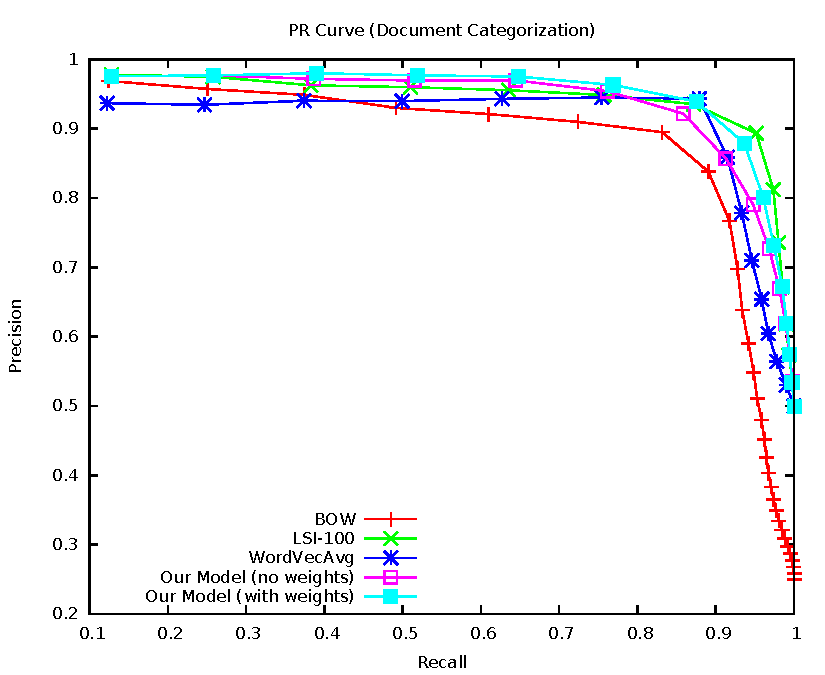
\includegraphics[width=0.7\columnwidth]{figs/pr/reuter-cs-scala.pdf}
        \vskip -4mm
    \caption{Precision/Recall for Document Categorization on Reuters-21578 (\emph{ModApte}) dataset} 
    \label{fig:pr:reuter:cs}
\end{figure}

%%%%%%%%%%%%%%%%%%%%%%%%%%%%%%%%%%%%%%%%%%%%%%  		Physics 		  %%%%%%%%%%%%%%%%%%%%%%%%%%%%%%%%%%%%%%%%%%%%%%%%%%%%%%%%%%%%%%%%%%%%%%%%%%%%%%%%%%%%%%%%%
\subsubsection{Physics - Wikipedia}
Performance of our model on the development data for different hyper-parameters is given in Tables~\ref{physics:hp:k}, ~\ref{physics:hp:epoch}, ~\ref{physics:hp:c} and ~\ref{physics:hp:n}. We find that our model gives the best performance for $k=100$ (Table~\ref{physics:hp:k}) when trained for $150$ epochs (Table~\ref{physics:hp:epoch}). Table~\ref{physics:hp:c} shows that larger context window ($c = 3$) and default number of negative samples ($n = 10$) per positive sample gives the best performance. 

\begin{table}[h!]
\tabcolsep=0.1cm
\footnotesize
\begin{center}
\begin{tabular}{l@{\hskip5mm} c c@{\hskip4mm} c@{\hskip5mm} c c@{\hskip4mm} c@{\hskip5mm} c c@{\hskip4mm} c}
\toprule
& \multicolumn{9}{c}{\textbf{Hyper-parameters} : {$epochs = 50$, $c = 2$, $n = 10$}}         \\
\cmidrule(lr){2-10}
\textbf{Tuning}
& \multicolumn{3}{c}{{$k = 50$}}         
& \multicolumn{3}{c}{{$k = 100$}}        
& \multicolumn{3}{c}{{$k = 150$}}        	\\
\cmidrule(lr){2-4}
\cmidrule(lr){5-7}
\cmidrule(lr){8-10}
%\cmidrule(lr){2-10}
\multirow{2}{*}{\textbf{Physics} (Development)}
& {P} & {R} & \textbf{F1} 
& {P} & {R} & \textbf{F1} 
& {P} & {R} & \textbf{F1} \\
\cmidrule(lr){2-4}
\cmidrule(lr){5-7}
\cmidrule(lr){8-10}
& 84.4   & 72.1  & 77.8
& 89.1   & 71.2  & \highest{79.2}
& 89.1   & 69.7  & 78.2 \\
\bottomrule         
\end{tabular}
%\vskip -4mm
\caption{\label{physics:hp:k} Model performance on Physics(Wikipedia) development data for different embedding dimensionality}
\end{center}
\end{table}

\begin{table}[h!]
\tabcolsep=0.1cm
\footnotesize
\begin{center}
\begin{tabular}{l c c c c c c c c c c c c c c c}
\toprule
& \multicolumn{15}{c}{\textbf{Hyper-parameters} : {$k = 100$, $c = 2$, $n = 10$}}         \\
\cmidrule(lr){2-16}
\textbf{Tuning}
& \multicolumn{3}{c}{{$epochs = 20$}}         
& \multicolumn{3}{c}{{$epochs = 50$}}         
& \multicolumn{3}{c}{{$epochs = 100$}}         
& \multicolumn{3}{c}{{$epochs = 150$}}         
& \multicolumn{3}{c}{{$epochs = 200$}}	\\
\cmidrule(lr){2-4}
\cmidrule(lr){5-7}
\cmidrule(lr){8-10}
\cmidrule(lr){11-13}
\cmidrule(lr){14-16}
\multirow{2}{*}{\textbf{Physics} (Development)}
& {P} & {R} & \textbf{F1} 
& {P} & {R} & \textbf{F1} 
& {P} & {R} & \textbf{F1} 
& {P} & {R} & \textbf{F1} 
& {P} & {R} & \textbf{F1} \\
\cmidrule(lr){2-4}
\cmidrule(lr){5-7}
\cmidrule(lr){8-10}
\cmidrule(lr){11-13}
\cmidrule(lr){14-16}
& 85.5   & 70.6  & 77.3
& 89.1   & 71.2  & 79.2
& 86.9   & 73.8  & 79.9
& 87.4   & 73.6  & \highest{79.9}
& 86.9   & 73.3  & 79.5 \\
\bottomrule         
\end{tabular}
\caption{\label{physics:hp:epoch} Model performance on Physics(Wikipedia) development data for different number of epochs}
%\vskip -4mm
\end{center}
\end{table}

\begin{table}[h!]
\tabcolsep=0.1cm
\footnotesize
\begin{center}
\begin{tabular}{l@{\hskip5mm} c c@{\hskip4mm} c@{\hskip5mm} c c@{\hskip4mm} c@{\hskip5mm} c c@{\hskip4mm} c}
\toprule
& \multicolumn{9}{c}{\textbf{Hyper-parameters} : {$k = 100$, $epochs = 150$, $n = 10$}}         \\
\cmidrule(lr){2-10}
\textbf{Tuning}
& \multicolumn{3}{c}{{$c = 2$}}         
& \multicolumn{3}{c}{{$c = 3$}}        
& \multicolumn{3}{c}{{$c = 4$}}        	\\
\cmidrule(lr){2-4}
\cmidrule(lr){5-7}
\cmidrule(lr){8-10}
%\cmidrule(lr){2-10}
\multirow{2}{*}{\textbf{Physics} (Development)}
& {P} & {R} & \textbf{F1} 
& {P} & {R} & \textbf{F1} 
& {P} & {R} & \textbf{F1} \\
\cmidrule(lr){2-4}
\cmidrule(lr){5-7}
\cmidrule(lr){8-10}
& 87.4   & 73.6  & 79.9
& 86.5   & 74.4  & \highest{80.0}
& 87.0   & 73.1  & 79.5 \\
\bottomrule         
\end{tabular}
%\vskip -4mm
\caption{\label{physics:hp:c} Model performance on Physics(Wikipedia) development data for different window sizes}
\end{center}
\end{table}

\begin{table}[h!]
\tabcolsep=0.1cm
\footnotesize
\begin{center}
\begin{tabular}{l@{\hskip5mm} c c@{\hskip4mm} c@{\hskip5mm} c c@{\hskip4mm} c@{\hskip5mm} c c@{\hskip4mm} c}
\toprule
& \multicolumn{9}{c}{\textbf{Hyper-parameters} : {$k = 100$, $epochs = 150$, $c = 3$}}         \\
\cmidrule(lr){2-10}
\textbf{Tuning}
& \multicolumn{3}{c}{{$n = 5$}}         
& \multicolumn{3}{c}{{$n = 10$}}        
& \multicolumn{3}{c}{{$n = 15$}}        	\\
\cmidrule(lr){2-4}
\cmidrule(lr){5-7}
\cmidrule(lr){8-10}
%\cmidrule(lr){2-10}
\multirow{2}{*}{\textbf{Physics} (Development)}
& {P} & {R} & \textbf{F1} 
& {P} & {R} & \textbf{F1} 
& {P} & {R} & \textbf{F1} \\
\cmidrule(lr){2-4}
\cmidrule(lr){5-7}
\cmidrule(lr){8-10}
& 85.5   & 74.3  & 79.5
& 86.5   & 74.4  & \highest{80.0}
& 87.8   & 73.3  & 79.9 \\
\bottomrule         
\end{tabular}
%\vskip -4mm
\caption{\label{physics:hp:n} Model performance on Physics(Wikipedia) development data for different number of negative samples}
\end{center}
\end{table}

Table~\ref{physics:cs} shows that our model outperforms other baseline models with a huge margin. 
Our model achieves a F1 score of $79.7\%$ while the second best model, \textbf{BOW} trails ours by $2.31\%$.
As observed in the evaluation of Reuters-21578, context weighing is necessary to learn high quality document representations. This is shown by the fact that when we simply sum the word vectors to represent the context, our model only achieves an accuracy of $73.8\%$ in terms of the F1 score.
Fig.~\ref{fig:pr:physics:cs} also shows that our model performs the best while \textbf{BOW} model is the second best performing model.

\begin{table}[h!]
\tabcolsep=0.1cm
\footnotesize
\begin{center}
\begin{tabular}{l@{\hskip5mm} c c@{\hskip4mm} c}
\toprule
% & \multicolumn{3}{c}{Reuters-21578}         \\
% \cmidrule(lr){2-4}
\textbf{Physics (Wikipedia)} & {P} & {R} & \textbf{F1} \\
\midrule
\textbf{BOW}
& 87.8   & 70.1  & 77.9 \\
\textbf{LSI-100}
& 83.4   & 69.5  & 75.8 \\
\textbf{WordVecAvg}
& 91.0   & 59.1  & 71.7 \\ \addlinespace[1mm]

\textbf{Our Model}
& \multirow{2}{*}{86.1}   & \multirow{2}{*}{64.6}  & \multirow{2}{*}{73.8} \\
(no weights) & & & \\ \addlinespace[1mm]
\textbf{Our Model}
& \multirow{2}{*}{88.6}   & \multirow{2}{*}{72.4}  & \multirow{2}{*}{\highest{79.7}} \\
(with weights) & & & \\
\bottomrule         
\end{tabular}
%\vskip -4mm
\caption{\label{physics:cs} Precision/Recall/F1 for Document Categorization on Physics(Wikipedia) dataset}
\end{center}
\end{table}

\begin{figure}[tb]
\centering
        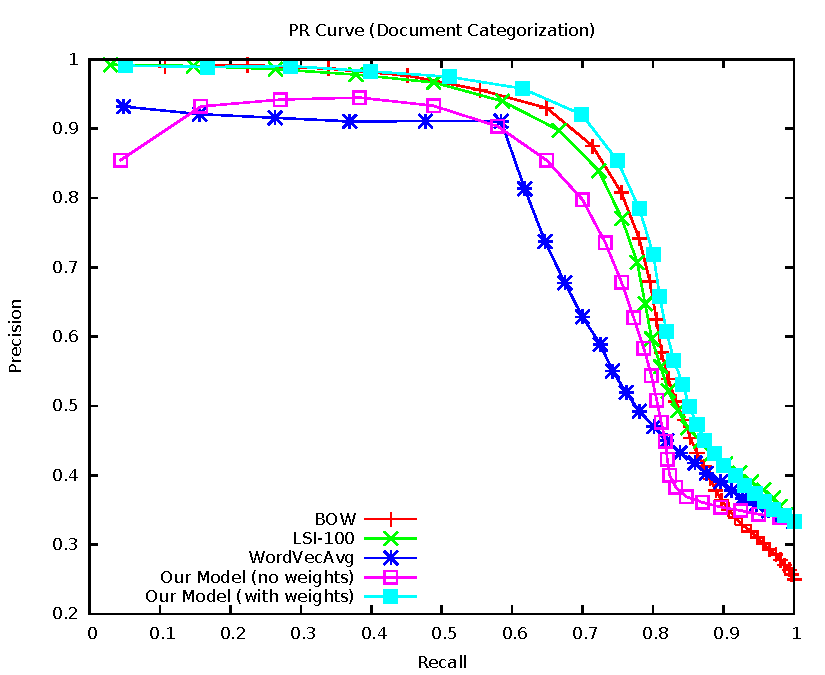
\includegraphics[width=0.7\columnwidth]{figs/pr/physics-cs-scala.pdf}
        \vskip -4mm
    \caption{ Precision/Recall for Document Categorization on Physics(Wikipedia) dataset}
    \label{fig:pr:physics:cs} 
\end{figure}

%%%%%%%%%%%%%%%%%%%%%%%%%%%%%%%%%%%%%%%%%%%%%%  		Biology 		  %%%%%%%%%%%%%%%%%%%%%%%%%%%%%%%%%%%%%%%%%%%%%%%%%%%%%%%%%%%%%%%%%%%%%%%%%%%%%%%%%%%%%%%%%
\subsubsection{Biology - Wikipedia}
The performance of our model on the development data for different values of hyper-parameters is shown in Tables~\ref{biology:hp:k}, ~\ref{biology:hp:epoch}, ~\ref{biology:hp:c} and ~\ref{biology:hp:n}. Table~\ref{biology:hp:k} shows that default embedding size of $k = 100$ performs best and relatively low training epochs ($epochs = 50$) gives the best results (Table~\ref{biology:hp:epoch}). Larger context window ($c = 3$) (Table~\ref{biology:hp:c}) and default number of negative samples ($n = 10$) per positive sample (Table~\ref{biology:hp:n}) gives the best model performance. 

\begin{table}[h!]
\tabcolsep=0.1cm
\footnotesize
\begin{center}
\begin{tabular}{l@{\hskip5mm} c c@{\hskip4mm} c@{\hskip5mm} c c@{\hskip4mm} c@{\hskip5mm} c c@{\hskip4mm} c}
\toprule
& \multicolumn{9}{c}{\textbf{Hyper-parameters} : {$epochs = 50$, $c = 2$, $n = 10$}}         \\
\cmidrule(lr){2-10}
\textbf{Tuning}
& \multicolumn{3}{c}{{$k = 50$}}         
& \multicolumn{3}{c}{{$k = 100$}}        
& \multicolumn{3}{c}{{$k = 150$}}        	\\
\cmidrule(lr){2-4}
\cmidrule(lr){5-7}
\cmidrule(lr){8-10}
%\cmidrule(lr){2-10}
\multirow{2}{*}{\textbf{Biology} (Development)}
& {P} & {R} & \textbf{F1} 
& {P} & {R} & \textbf{F1} 
& {P} & {R} & \textbf{F1} \\
\cmidrule(lr){2-4}
\cmidrule(lr){5-7}
\cmidrule(lr){8-10}
& 83.9   & 60.0  & 70.0
& 82.4   & 61.2  & \highest{70.2}
& 83.7   & 60.2  & 70.0 \\
\bottomrule         
\end{tabular}
%\vskip -4mm
\caption{\label{biology:hp:k} Model performance on Biology(Wikipedia) development data for different embedding dimensionality}
\end{center}
\end{table}

\begin{table}[tb]
\tabcolsep=0.1cm
\footnotesize
\begin{center}
\begin{tabular}{l c c c c c c c c c c c c c c c}
\toprule
& \multicolumn{15}{c}{\textbf{Hyper-parameters} : {$k = 100$, $c = 2$, $n = 10$}}         \\
\cmidrule(lr){2-16}
\textbf{Tuning}
& \multicolumn{3}{c}{{$epochs = 20$}}         
& \multicolumn{3}{c}{{$epochs = 50$}}         
& \multicolumn{3}{c}{{$epochs = 100$}}         
& \multicolumn{3}{c}{{$epochs = 150$}}         
& \multicolumn{3}{c}{{$epochs = 200$}}	\\
\cmidrule(lr){2-4}
\cmidrule(lr){5-7}
\cmidrule(lr){8-10}
\cmidrule(lr){11-13}
\cmidrule(lr){14-16}
\multirow{2}{*}{\textbf{Biology} (Development)}
& {P} & {R} & \textbf{F1} 
& {P} & {R} & \textbf{F1} 
& {P} & {R} & \textbf{F1} 
& {P} & {R} & \textbf{F1} 
& {P} & {R} & \textbf{F1} \\
\cmidrule(lr){2-4}
\cmidrule(lr){5-7}
\cmidrule(lr){8-10}
\cmidrule(lr){11-13}
\cmidrule(lr){14-16}
& 75.3   & 59.8  & 66.7
& 82.4   & 61.2  & \highest{70.2}
& 82.9   & 60.2  & 69.7
& 85.6   & 58.6  & 69.6
& 85.3   & 58.0  & 69.0 \\
\bottomrule         
\end{tabular}
\caption{\label{biology:hp:epoch} Model performance on Biology(Wikipedia) development data for different number of epochs}
%\vskip -4mm
\end{center}
\end{table}

\begin{table}[h!]
\tabcolsep=0.1cm
\footnotesize
\begin{center}
\begin{tabular}{l@{\hskip5mm} c c@{\hskip4mm} c@{\hskip5mm} c c@{\hskip4mm} c@{\hskip5mm} c c@{\hskip4mm} c}
\toprule
& \multicolumn{9}{c}{\textbf{Hyper-parameters} : {$k = 100$, $epochs = 50$, $n = 10$}}         \\
\cmidrule(lr){2-10}
\textbf{Tuning}
& \multicolumn{3}{c}{{$c = 2$}}         
& \multicolumn{3}{c}{{$c = 3$}}        
& \multicolumn{3}{c}{{$c = 4$}}        	\\
\cmidrule(lr){2-4}
\cmidrule(lr){5-7}
\cmidrule(lr){8-10}
%\cmidrule(lr){2-10}
\multirow{2}{*}{\textbf{Biology} (Development)}
& {P} & {R} & \textbf{F1} 
& {P} & {R} & \textbf{F1} 
& {P} & {R} & \textbf{F1} \\
\cmidrule(lr){2-4}
\cmidrule(lr){5-7}
\cmidrule(lr){8-10}
& 82.4   & 61.2  & \highest{70.2}
& 80.8   & 62.0  & \highest{70.2}
& 81.3   & 61.4  & 70.0 \\
\bottomrule         
\end{tabular}
%\vskip -4mm
\caption{\label{biology:hp:c}Model performance on Biology(Wikipedia) development data for different window sizes}
\end{center}
\end{table}

\begin{table}[h!]
\tabcolsep=0.1cm
\footnotesize
\begin{center}
\begin{tabular}{l@{\hskip5mm} c c@{\hskip4mm} c@{\hskip5mm} c c@{\hskip4mm} c@{\hskip5mm} c c@{\hskip4mm} c}
\toprule
& \multicolumn{9}{c}{\textbf{Hyper-parameters} : {$k = 100$, $epochs = 50$, $c = 3$}}         \\
\cmidrule(lr){2-10}
\textbf{Tuning}
& \multicolumn{3}{c}{{$n = 5$}}         
& \multicolumn{3}{c}{{$n = 10$}}        
& \multicolumn{3}{c}{{$n = 15$}}        	\\
\cmidrule(lr){2-4}
\cmidrule(lr){5-7}
\cmidrule(lr){8-10}
%\cmidrule(lr){2-10}
\multirow{2}{*}{\textbf{Biology} (Development)}
& {P} & {R} & \textbf{F1} 
& {P} & {R} & \textbf{F1} 
& {P} & {R} & \textbf{F1} \\
\cmidrule(lr){2-4}
\cmidrule(lr){5-7}
\cmidrule(lr){8-10}
& 81.8   & 61.0  & 69.9
& 80.8   & 62.0  & \highest{70.2}
& 81.2   & 60.8  & 69.6 \\
\bottomrule         
\end{tabular}
%\vskip -4mm
\caption{\label{biology:hp:n}Model performance on Biology(Wikipedia) development data for different number of negative samples}
\end{center}
\end{table}

Table~\ref{biology:cs} shows that the distributed representations learned by our model outperform some baseline representations but the bag-of-words representation works the best.
Our model achieves a F1 score of $67.8\%$ while the \textbf{BOW} improves our model by $1.7\%$.
The model accuracy suffers by $4.95\%$ when context word weighting is ignored during training. We also find that document representations learned by averaging word vectors performs the worst.
Fig.~\ref{fig:pr:biology:cs} shows the precision/recall curves for our model and other baseline methods. It also shows that the \textbf{BOW} representations perform the closest to representations learned using our model.

\begin{table}[h!]
\tabcolsep=0.1cm
\footnotesize
\begin{center}
\begin{tabular}{l@{\hskip5mm} c c@{\hskip4mm} c}
\toprule
% & \multicolumn{3}{c}{Reuters-21578}         \\
% \cmidrule(lr){2-4}
\textbf{Biology (Wikipedia)} & {P} & {R} & \textbf{F1} \\
\midrule
\textbf{BOW}
& 90.3   & 59.5  & \highest{69.0} \\
\textbf{LSI-100}
& 82.1   & 51.6  & 63.4 \\
\textbf{WordVecAvg}
& 79.4   & 50.4  & 61.6 \\ \addlinespace[1mm]

\textbf{Our Model}
& \multirow{2}{*}{80.3}   & \multirow{2}{*}{53.8}  & \multirow{2}{*}{64.4} \\
(no weights) & & & \\ \addlinespace[1mm]
\textbf{Our Model}
& \multirow{2}{*}{79.7}   & \multirow{2}{*}{59.0}  & \multirow{2}{*}{67.8} \\
(with weights) & & & \\
\bottomrule         
\end{tabular}
%\vskip -4mm
\caption{\label{biology:cs} Precision/Recall/F1 for Document Categorization on Biology(Wikipedia) dataset}
\end{center}
\end{table}

\begin{figure}[tb]
\centering
        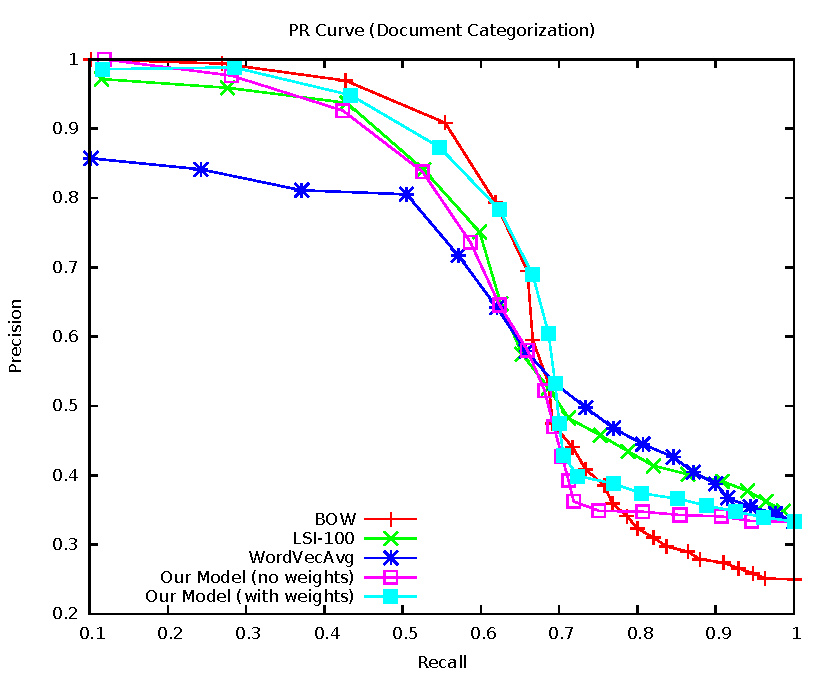
\includegraphics[width=0.7\columnwidth]{figs/pr/biology-cs-scala.pdf}
        \vskip -4mm
    \caption{ Precision/Recall for Document Categorization on Biology(Wikipedia) dataset}
    \label{fig:pr:biology:cs} 
\end{figure}

%%%%%%%%%%%%%%%%%%%%%%%%%%%%%%%%%%%%%%%%%%%%%%  		Mathematics 		  %%%%%%%%%%%%%%%%%%%%%%%%%%%%%%%%%%%%%%%%%%%%%%%%%%%%%%%%%%%%%%%%%%%%%%%%%%%%%%%%%%%%%%%%%
\subsubsection{Mathematics - Wikipedia}
Tables~\ref{mathematics:hp:k}, ~\ref{mathematics:hp:epoch}, ~\ref{mathematics:hp:c} and ~\ref{mathematics:hp:n} show that low embedding size of $k = 50$ and moderate training epochs ($epochs = 100$) give the best model performance. We also find that relatively larger context window ($c = 3$) and number of negative samples ($n = 15$) per positive sample are required for optimal model performance.

\begin{table}[h!]
\tabcolsep=0.1cm
\footnotesize
\begin{center}
\begin{tabular}{l@{\hskip5mm} c c@{\hskip4mm} c@{\hskip5mm} c c@{\hskip4mm} c@{\hskip5mm} c c@{\hskip4mm} c}
\toprule
& \multicolumn{9}{c}{\textbf{Hyper-parameters} : {$epochs = 50$, $c = 2$, $n = 10$}}         \\
\cmidrule(lr){2-10}
\textbf{Tuning}
& \multicolumn{3}{c}{{$k = 50$}}         
& \multicolumn{3}{c}{{$k = 100$}}        
& \multicolumn{3}{c}{{$k = 150$}}        	\\
\cmidrule(lr){2-4}
\cmidrule(lr){5-7}
\cmidrule(lr){8-10}
%\cmidrule(lr){2-10}
\multirow{2}{*}{\textbf{Mathematics} (Development)}
& {P} & {R} & \textbf{F1} 
& {P} & {R} & \textbf{F1} 
& {P} & {R} & \textbf{F1} \\
\cmidrule(lr){2-4}
\cmidrule(lr){5-7}
\cmidrule(lr){8-10}
& 83.2   & 57.0  & \highest{67.7}
& 82.3   & 56.0  & 66.7
& 86.1   & 55.5  & 67.5 \\
\bottomrule         
\end{tabular}
%\vskip -4mm
\caption{\label{mathematics:hp:k} Model performance on Mathematics(Wikipedia) development data for different embedding dimensionality}
\end{center}
\end{table}

\begin{table}[h!]
\tabcolsep=0.1cm
\footnotesize
\begin{center}
\begin{tabular}{l c c c c c c c c c c c c c c c}
\toprule
& \multicolumn{15}{c}{\textbf{Hyper-parameters} : {$k = 50$, $c = 2$, $n = 10$}}         \\
\cmidrule(lr){2-16}
\textbf{Tuning}
& \multicolumn{3}{c}{{$epochs = 20$}}         
& \multicolumn{3}{c}{{$epochs = 50$}}         
& \multicolumn{3}{c}{{$epochs = 100$}}         
& \multicolumn{3}{c}{{$epochs = 150$}}         
& \multicolumn{3}{c}{{$epochs = 200$}}	\\
\cmidrule(lr){2-4}
\cmidrule(lr){5-7}
\cmidrule(lr){8-10}
\cmidrule(lr){11-13}
\cmidrule(lr){14-16}
\multirow{2}{*}{\textbf{Mathematics} (Development)}
& {P} & {R} & \textbf{F1} 
& {P} & {R} & \textbf{F1} 
& {P} & {R} & \textbf{F1} 
& {P} & {R} & \textbf{F1} 
& {P} & {R} & \textbf{F1} \\
\cmidrule(lr){2-4}
\cmidrule(lr){5-7}
\cmidrule(lr){8-10}
\cmidrule(lr){11-13}
\cmidrule(lr){14-16}
& 81.2   & 55.2  & 65.8
& 83.2   & 57.0  & 67.7
& 87.0   & 56.3  & \highest{68.3}
& 86.7   & 55.2  & 67.5
& 82.2   & 57.8  & 67.9 \\
\bottomrule         
\end{tabular}
\caption{\label{mathematics:hp:epoch} Model performance on Mathematics(Wikipedia) development data for different number of epochs}
%\vskip -4mm
\end{center}
\end{table}

\begin{table}[h!]
\tabcolsep=0.1cm
\footnotesize
\begin{center}
\begin{tabular}{l@{\hskip5mm} c c@{\hskip4mm} c@{\hskip5mm} c c@{\hskip4mm} c@{\hskip5mm} c c@{\hskip4mm} c}
\toprule
& \multicolumn{9}{c}{\textbf{Hyper-parameters} : {$k = 50$, $epochs = 100$, $n = 10$}}         \\
\cmidrule(lr){2-10}
\textbf{Tuning}
& \multicolumn{3}{c}{{$c = 2$}}         
& \multicolumn{3}{c}{{$c = 3$}}        
& \multicolumn{3}{c}{{$c = 4$}}        	\\
\cmidrule(lr){2-4}
\cmidrule(lr){5-7}
\cmidrule(lr){8-10}
%\cmidrule(lr){2-10}
\multirow{2}{*}{\textbf{Mathematics} (Development)}
& {P} & {R} & \textbf{F1} 
& {P} & {R} & \textbf{F1} 
& {P} & {R} & \textbf{F1} \\
\cmidrule(lr){2-4}
\cmidrule(lr){5-7}
\cmidrule(lr){8-10}
& 87.0   & 56.3  & \highest{68.3}
& 91.0   & 54.5  & 68.2
& 88.1   & 55.0  & 67.7 \\
\bottomrule         
\end{tabular}
%\vskip -4mm
\caption{\label{mathematics:hp:c} Model performance on Mathematics(Wikipedia) development data for different window sizes}
\end{center}
\end{table}

\begin{table}[h!]
\tabcolsep=0.1cm
\footnotesize
\begin{center}
\begin{tabular}{l@{\hskip5mm} c c@{\hskip4mm} c@{\hskip5mm} c c@{\hskip4mm} c@{\hskip5mm} c c@{\hskip4mm} c}
\toprule
& \multicolumn{9}{c}{\textbf{Hyper-parameters} : {$k = 50$, $epochs = 100$, $c = 2$}}         \\
\cmidrule(lr){2-10}
\textbf{Tuning}
& \multicolumn{3}{c}{{$n = 5$}}         
& \multicolumn{3}{c}{{$n = 10$}}        
& \multicolumn{3}{c}{{$n = 15$}}        	\\
\cmidrule(lr){2-4}
\cmidrule(lr){5-7}
\cmidrule(lr){8-10}
%\cmidrule(lr){2-10}
\multirow{2}{*}{\textbf{Mathematics} (Development)}
& {P} & {R} & \textbf{F1} 
& {P} & {R} & \textbf{F1} 
& {P} & {R} & \textbf{F1} \\
\cmidrule(lr){2-4}
\cmidrule(lr){5-7}
\cmidrule(lr){8-10}
& 86.1   & 57.0  & 68.6
& 87.0   & 56.3  & 68.3
& 90.0   & 55.5  & \highest{68.7} \\
\bottomrule         
\end{tabular}
%\vskip -4mm
\caption{\label{mathematics:hp:n} Model performance on Mathematics(Wikipedia) development data for different number of negative samples}
\end{center}
\end{table}

Table~\ref{mathematics:cs} shows that the distributed representations learned by our model outperform other baseline representations.
Our model achieves a F1 score of $68.2\%$ while the second best model, \textbf{BOW} trails ours by $4.41\%$.
Word vectors averaged by tf-idf weighing scheme to represent document in the Mathematics (Wikipedia) dataset give the worst accuracy with an F1 score of $55.7\%$.
We again find that context word weighing when computing the project layer is important and gives the best performance.
Fig.~\ref{fig:pr:mathematics:cs} shows the precision/recall curves for our model and other baseline methods. 

\begin{table}[h!]
\tabcolsep=0.1cm
\footnotesize
\begin{center}
\begin{tabular}{l@{\hskip5mm} c c@{\hskip4mm} c}
\toprule
% & \multicolumn{3}{c}{Reuters-21578}         \\
% \cmidrule(lr){2-4}
\textbf{Mathematics (Wikipedia)} & {P} & {R} & \textbf{F1} \\
\midrule
\textbf{BOW}
& 65.6   & 65.1  & 65.3 \\
\textbf{LSI-100}
& 89.7   & 50.3  & 64.4 \\
\textbf{WordVecAvg}
& 90.5   & 40.3  & 55.7 \\ \addlinespace[1mm]

\textbf{Our Model}
& \multirow{2}{*}{78.4}   & \multirow{2}{*}{57.4}  & \multirow{2}{*}{66.3} \\
(no weights) & & & \\ \addlinespace[1mm]
\textbf{Our Model}
& \multirow{2}{*}{85.3}   & \multirow{2}{*}{56.8}  & \multirow{2}{*}{\highest{68.2}} \\
(with weights) & & & \\
\bottomrule         
\end{tabular}
%\vskip -4mm
\caption{\label{mathematics:cs} Precision/Recall/F1 for Document Categorization on Mathematics(Wikipedia) dataset}
\end{center}
\end{table}

\begin{figure}[tb]
\centering
        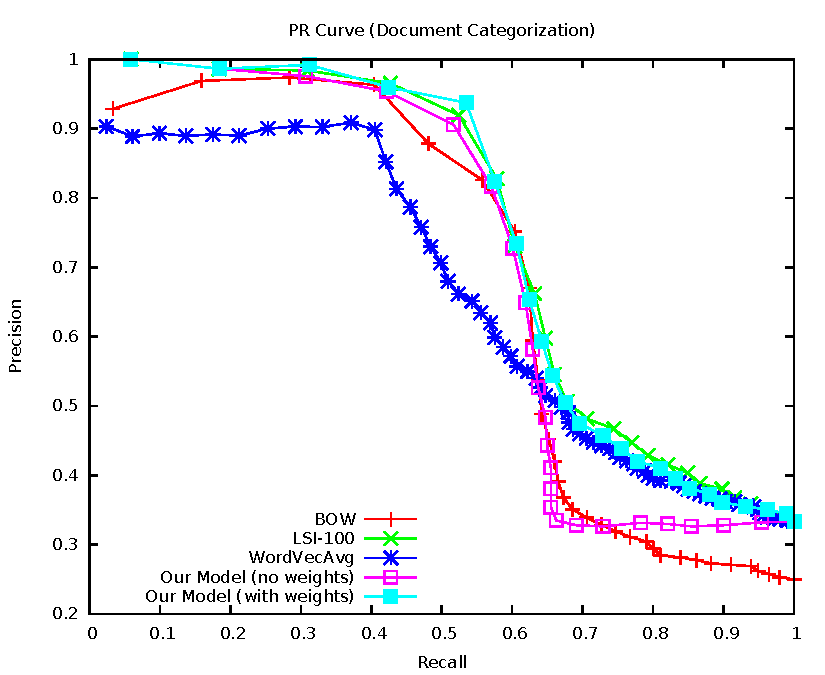
\includegraphics[width=0.7\columnwidth]{figs/pr/mathematics-cs-scala.pdf}
        \vskip -4mm
    \caption{ Precision/Recall for Document Categorization on Mathematics(Wikipedia) dataset}
    \label{fig:pr:mathematics:cs} 
\end{figure}

%%%%%%%%%%%%%%%%%%%%%%%%%%%%%%%%%%%%%%%%%%%%%%  		Sports 		  %%%%%%%%%%%%%%%%%%%%%%%%%%%%%%%%%%%%%%%%%%%%%%%%%%%%%%%%%%%%%%%%%%%%%%%%%%%%%%%%%%%%%%%%%
\subsubsection{Sports - Wikipedia}
The performance of our model on the development data for different values of different hyper-parameters is shown in Tables~\ref{sports:hp:k}, ~\ref{sports:hp:epoch}, ~\ref{sports:hp:c} and ~\ref{sports:hp:n}. Table~\ref{sports:hp:k} shows that low vector size of $k = 50$ and Table~\ref{sports:hp:epoch} shows moderate training epochs ($epochs = 100$) gives the best model performance. 
Table~\ref{sports:hp:c} shows that context window size of $c = 3$ and relatively larger number of negative samples ($n = 15$) per positive sample achieves the best performance.

\begin{table}[h!]
\tabcolsep=0.1cm
\footnotesize
\begin{center}
\begin{tabular}{l@{\hskip5mm} c c@{\hskip4mm} c@{\hskip5mm} c c@{\hskip4mm} c@{\hskip5mm} c c@{\hskip4mm} c}
\toprule
& \multicolumn{9}{c}{\textbf{Hyper-parameters} : {$epochs = 50$, $c = 2$, $n = 10$}}         \\
\cmidrule(lr){2-10}
\textbf{Tuning}
& \multicolumn{3}{c}{{$k = 50$}}         
& \multicolumn{3}{c}{{$k = 100$}}        
& \multicolumn{3}{c}{{$k = 150$}}        	\\
\cmidrule(lr){2-4}
\cmidrule(lr){5-7}
\cmidrule(lr){8-10}
%\cmidrule(lr){2-10}
\multirow{2}{*}{\textbf{Sports} (Development)}
& {P} & {R} & \textbf{F1} 
& {P} & {R} & \textbf{F1} 
& {P} & {R} & \textbf{F1} \\
\cmidrule(lr){2-4}
\cmidrule(lr){5-7}
\cmidrule(lr){8-10}
& 82.2   & 45.7  & \highest{58.8}
& 81.2   & 45.9  & 58.6
& 80.9   & 45.7  & 58.4 \\
\bottomrule         
\end{tabular}
%\vskip -4mm
\caption{\label{sports:hp:k} Model performance on Sports(Wikipedia) development data for different embedding dimensionality}
\end{center}
\end{table}

\begin{table}[tb]
\tabcolsep=0.1cm
\footnotesize
\begin{center}
\begin{tabular}{l c c c c c c c c c c c c c c c}
\toprule
& \multicolumn{15}{c}{\textbf{Hyper-parameters} : {$k = 50$, $c = 2$, $n = 10$}}         \\
\cmidrule(lr){2-16}
\textbf{Tuning}
& \multicolumn{3}{c}{{$epochs = 20$}}         
& \multicolumn{3}{c}{{$epochs = 50$}}         
& \multicolumn{3}{c}{{$epochs = 100$}}         
& \multicolumn{3}{c}{{$epochs = 150$}}         
& \multicolumn{3}{c}{{$epochs = 200$}}	\\
\cmidrule(lr){2-4}
\cmidrule(lr){5-7}
\cmidrule(lr){8-10}
\cmidrule(lr){11-13}
\cmidrule(lr){14-16}
\multirow{2}{*}{\textbf{Sports} (Development)}
& {P} & {R} & \textbf{F1} 
& {P} & {R} & \textbf{F1} 
& {P} & {R} & \textbf{F1} 
& {P} & {R} & \textbf{F1} 
& {P} & {R} & \textbf{F1} \\
\cmidrule(lr){2-4}
\cmidrule(lr){5-7}
\cmidrule(lr){8-10}
\cmidrule(lr){11-13}
\cmidrule(lr){14-16}
& 73.9   & 45.9  & 56.6
& 82.2   & 45.7  & 58.8
& 83.9   & 47.6  & \highest{60.7}
& 83.7   & 46.8  & 60.0
& 67.1   & 50.2  & 57.4 \\
\bottomrule         
\end{tabular}
\caption{\label{sports:hp:epoch}  Model performance on Sports(Wikipedia) development data for different number of epochs}
%\vskip -4mm
\end{center}
\end{table}

\begin{table}[h!]
\tabcolsep=0.1cm
\footnotesize
\begin{center}
\begin{tabular}{l@{\hskip5mm} c c@{\hskip4mm} c@{\hskip5mm} c c@{\hskip4mm} c@{\hskip5mm} c c@{\hskip4mm} c}
\toprule
& \multicolumn{9}{c}{\textbf{Hyper-parameters} : {$k = 50$, $epochs = 100$, $n = 10$}}         \\
\cmidrule(lr){2-10}
\textbf{Tuning}
& \multicolumn{3}{c}{{$c = 2$}}         
& \multicolumn{3}{c}{{$c = 3$}}        
& \multicolumn{3}{c}{{$c = 4$}}        	\\
\cmidrule(lr){2-4}
\cmidrule(lr){5-7}
\cmidrule(lr){8-10}
%\cmidrule(lr){2-10}
\multirow{2}{*}{\textbf{Sports} (Development)}
& {P} & {R} & \textbf{F1} 
& {P} & {R} & \textbf{F1} 
& {P} & {R} & \textbf{F1} \\
\cmidrule(lr){2-4}
\cmidrule(lr){5-7}
\cmidrule(lr){8-10}
& 83.9   & 47.6  & 60.7
& 84.5   & 47.8  & \highest{61.0}
& 86.0   & 47.0  & 60.8 \\
\bottomrule         
\end{tabular}
%\vskip -4mm
\caption{\label{sports:hp:c} Model performance on Sports(Wikipedia) development data for different window sizes}
\end{center}
\end{table}

\begin{table}[h!]
\tabcolsep=0.1cm
\footnotesize
\begin{center}
\begin{tabular}{l@{\hskip5mm} c c@{\hskip4mm} c@{\hskip5mm} c c@{\hskip4mm} c@{\hskip5mm} c c@{\hskip4mm} c}
\toprule
& \multicolumn{9}{c}{\textbf{Hyper-parameters} : {$k = 50$, $epochs = 100$, $c = 3$}}         \\
\cmidrule(lr){2-10}
\textbf{Tuning}
& \multicolumn{3}{c}{{$n = 5$}}         
& \multicolumn{3}{c}{{$n = 10$}}        
& \multicolumn{3}{c}{{$n = 15$}}        	\\
\cmidrule(lr){2-4}
\cmidrule(lr){5-7}
\cmidrule(lr){8-10}
%\cmidrule(lr){2-10}
\multirow{2}{*}{\textbf{Sports} (Development)}
& {P} & {R} & \textbf{F1} 
& {P} & {R} & \textbf{F1} 
& {P} & {R} & \textbf{F1} \\
\cmidrule(lr){2-4}
\cmidrule(lr){5-7}
\cmidrule(lr){8-10}
& 84.6   & 47.0  & 60.4
& 84.5   & 47.8  & \highest{61.0}
& 82.7   & 47.4  & 60.3 \\
\bottomrule         
\end{tabular}
%\vskip -4mm
\caption{\label{sports:hp:n} Model performance on Sports(Wikipedia) development data for different number of negative samples}
\end{center}
\end{table}

Table~\ref{sports:cs} shows that the distributed representations learned by our model outperform other baseline representations.
Our model achieves a F1 score of $57.3\%$ while again the \textbf{BOW} model is second best performing.
As found in previous evaluations, document representations using bag-of-words style word vector averaging perform the worst. 
Fig.~\ref{fig:pr:sports:cs} shows the precision/recall curves for our model and other baseline methods. 

\begin{table}[h!]
\tabcolsep=0.1cm
\footnotesize
\begin{center}
\begin{tabular}{l@{\hskip5mm} c c@{\hskip4mm} c}
\toprule
% & \multicolumn{3}{c}{Reuters-21578}         \\
% \cmidrule(lr){2-4}
\textbf{Sports (Wikipedia)} & {P} & {R} & \textbf{F1} \\
\midrule
\textbf{BOW}
& 91.7   & 41.3  & 56.9 \\
\textbf{LSI-100}
& 91.2   & 40.1  & 55.7 \\
\textbf{WordVecAvg}
& 81.8   & 37.5  & 51.4 \\ \addlinespace[1mm]

\textbf{Our Model}
& \multirow{2}{*}{80.5}   & \multirow{2}{*}{40.1}  & \multirow{2}{*}{53.6} \\
(no weights) & & & \\ \addlinespace[1mm]
\textbf{Our Model}
& \multirow{2}{*}{82.1}   & \multirow{2}{*}{44.0}  & \multirow{2}{*}{\highest{57.3}} \\
(with weights) & & & \\
\bottomrule         
\end{tabular}
%\vskip -4mm
\caption{\label{sports:cs} Precision/Recall/F1 for Document Categorization on Sports(Wikipedia) dataset}
\end{center}
\end{table}

\begin{figure}[tb]
\centering
        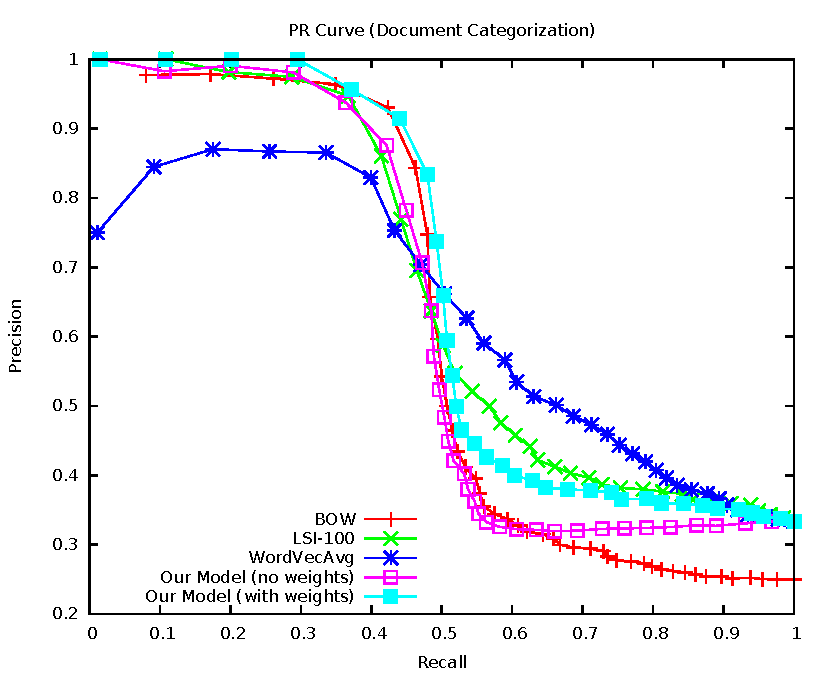
\includegraphics[width=0.7\columnwidth]{figs/pr/sports-cs-scala.pdf}
        \vskip -4mm
    \caption{Precision/Recall for Document Categorization on Sports(Wikipedia) dataset}
    \label{fig:pr:sports:cs} 
\end{figure}

%%%%%%%%%%%%%%%%%%%%%%%%%%%%%			IMPUTING MISSING CAEGORIES 				%%%%%%%%%%%%%%%%%%%%%%%%%%%%%%%%%%%%%%%%%%%%%%%%%%%%%%%%%%%%%%%%%%%%%%%%%%%%%%%%%%%%%%%%%%%%%%
\subsection{Imputing Missing Categories}
\label{sec:results:imputing}
Most of the real-life databases that contain categorization for documents contain incomplete information. In the case of huge number of categories and when document categorization is carried out by non-experts, as in Wikipedia, one can never be sure that all the relevant categories have been assigned to each document. In such large-scale databases where manual annotation and review is difficult, systems that can automatically impute missing categories for documents in the database are imperative.

In this section we evaluate our system's efficacy in imputing missing categories in the Wikipedia datasets.  
The task is similar to Relational Learning where the task is to complete the sparse relational matrix, $R$ between two types of entities. 
In our case, we estimate the probability of every unobserved document-category pair $(d_{i}, c_{k})$ to be true to complete the sparse document-category matrix in which only positive document-category pairs are observed.
For training and testing purposes, we first introduce corrupt document-category pairs as negative samples in the training data $\traindata$ in the following manner. For every positive $\{ d_{i}, c_{j}, 1\}$ observed in the training data, we introduce two negative samples $\{ d_{i}, c_{k}, 0\}$ where the negative sampled category $c'_{k}$ is chosen uniformly for the category set. This increases the tuples in the training data by three times. From the modified training data we randomly choose $80\%$ document-category pairs for training purposes and divide the rest equally for development and test purposes. The document representations are learned in the same manner as in the previous evaluation.

Table~\ref{wikipedia:ho} shows our model's efficacy in imputing missing categories in the different Wikipedia datasets. We also compute a combined F1 score for all the datasets in the micro-averaged fashion, i.e. by combining all the predictions for all the datasets and then computing the precision and recall. 
As expected our model of learning distributed document representations outperforms all other baselines by a large margin. 
Our model achieves an overall F1 score of $74.3\%$ which improves upon the bag-of-words (\textbf{BOW}) model by $4.78\%$. 
Representing documents by averaging the word vectors using \emph{tf-idf} weighing scheme achieves a F1 score of $65.4\%$. 
The worst performing model, as expected is \textbf{PMF} which does not use any textual information about the documents.
As found in the previous section, in our model, simple summing of context word vectors to represent the context does not provide competitive results which corroborates the hypothesis that encoding syntactic information is necessary. 
%Figure~\ref{fig:pr:wiki:ho} shows the precision/recall curves for the different document representation models along with the performance of our models.

\begin{table}[h!]
\tabcolsep=1mm
\footnotesize
\begin{center}
%\begin{tabular}{l cc@{\hskip 2mm}c@{\hskip 2mm} cc@{\hskip 2mm}c@{\hskip 2mm} cc@{\hskip 2mm}c@{\hskip 2mm} cc@{\hskip 2mm}c@{\hskip 2mm} cc@{\hskip 2mm}c}
\begin{tabular}{l ccc@{\hskip 3mm} ccc@{\hskip 3mm} ccc@{\hskip 3mm} ccc@{\hskip 3mm} ccc}
\toprule
\multirow{2}{*}{} & 
\multicolumn{3}{c}{{Physics}}         & 
\multicolumn{3}{c}{{Biology}}        & \multicolumn{3}{c}{{Mathematics}}         & \multicolumn{3}{c}{{Sports}}        & %\multicolumn{3}{c}{\textbf{Restaurant}}       & 
\multicolumn{3}{c}{\textbf{Combined}}              
\\ 
\cmidrule(lr){2-4}
\cmidrule(lr){5-7}
\cmidrule(lr){8-10}
\cmidrule(lr){11-13}
\cmidrule(lr){14-16}
& 
{P} & {R} & \textbf{F1} & 
{P} & {R} & \textbf{F1} & 
{P} & {R} & \textbf{F1} & 
{P} & {R} & \textbf{F1} &
{P} & {R} & \textbf{F1} \\ 
\midrule
\textbf{PMF}
& 73.0   & 64.3  & 68.4
& 72.1   & 47.5  & 57.3
& 41.6   & 58.2  & 48.5
& 51.3   & 35.6  & 42.0
& 63.0   & 54.8  & 58.6 
\\
\textbf{LSI-100}
& 59.5   & 82.3  & 69.0
& 49.9   & 71.6  & 58.8
& 47.1   & 73.0  & 57.3
& 43.1   & 68.2  & 52.8
& 52.5   & 76.3  & 62.2
\\ 
\textbf{BOW}
& 76.1   & 79.4  & 77.7
& 69.7   & 67.7  & 68.7
& 70.9   & 63.5  & 67.0
& 64.8   & 49.3  & 56.0
& 72.5   & 69.4  & 70.9
\\
\textbf{WordVecAvg}
& 88.0   & 63.5  & 73.8
& 80.7   & 50.3  & 61.9
& 71.8   & 46.7  & 56.6
& 87.2   & 35.4  & 50.3
& 84.2   & 53.4  & 65.4
\\ \addlinespace[1mm]
\textbf{Our Model}
& \multirow{2}{*}{88.6}   & \multirow{2}{*}{69.1}  & \multirow{2}{*}{77.7}
& \multirow{2}{*}{80.5}   & \multirow{2}{*}{55.3}  & \multirow{2}{*}{65.6}
& \multirow{2}{*}{74.3}   & \multirow{2}{*}{53.1}  & \multirow{2}{*}{61.9}
& \multirow{2}{*}{84.7}   & \multirow{2}{*}{40.2}  & \multirow{2}{*}{54.5}
& \multirow{2}{*}{85.4}   & \multirow{2}{*}{58.5}  & \multirow{2}{*}{69.2}
\\ 
(without weights) & & & & & & & & & & & & & &  & \\
\addlinespace[1mm]
\textbf{Our Model}
& \multirow{2}{*}{89.9}   & \multirow{2}{*}{74.5}  & \multirow{2}{*}{\highest{81.5}}
& \multirow{2}{*}{84.9}   & \multirow{2}{*}{63.8} & \multirow{2}{*}{\highest{72.9}}
& \multirow{2}{*}{79.9}   & \multirow{2}{*}{60.7}  & \multirow{2}{*}{\highest{69.0}}
& \multirow{2}{*}{81.1}   & \multirow{2}{*}{45.6} & \multirow{2}{*}{\highest{58.4}}
& \multirow{2}{*}{86.3}   & \multirow{2}{*}{65.2}  & \multirow{2}{*}{\highest{74.3}}
\\ 
(with weights) & & & & & & & & & & & & & &  & \\
\bottomrule         
\end{tabular}
\end{center}
\caption{\label{wikipedia:ho} Precision/Recall/F1 for Imputing Missing Categories in the Wikipedia Datasets }
\end{table}
% \begin{figure}[tb]
% \centering
%         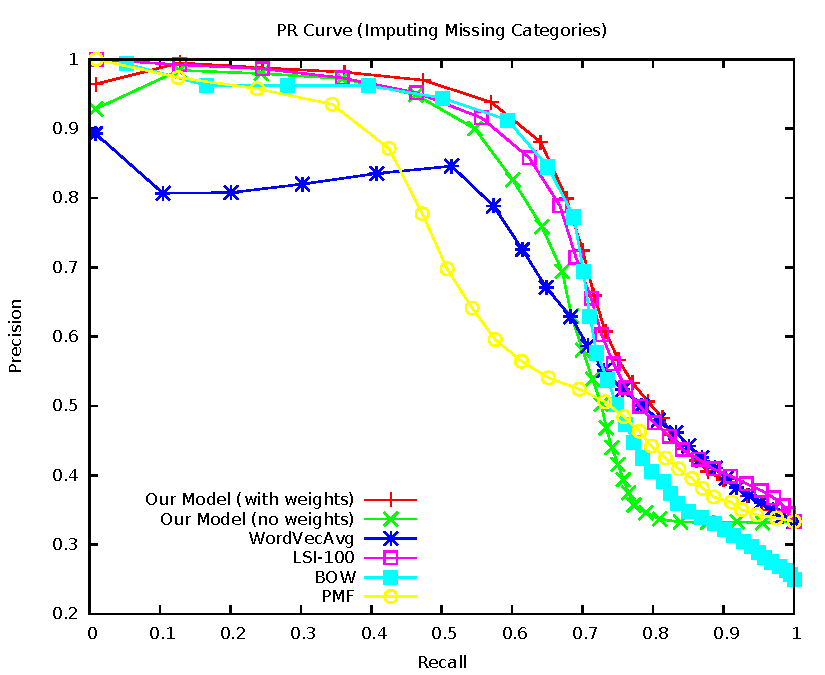
\includegraphics[width=0.8\columnwidth]{figs/pr/wiki-ho-scala.pdf}
%         \vskip -4mm
%     \caption{\footnotesize Precision/Recall for Imputing Missing Categories on the Wikipedia datasets}
%     \label{fig:pr:wiki:ho} 
% \end{figure}

\subsection{Estimating Similarity between Categories and Words}
One of the primary drawbacks faced by the bag-of-words representations is the lack of similarity measures due to the discrete nature of the representation vectors. 
Also, when documents are represented using bag-of-words vectors, there is no representation for the words in the vocabulary. 
As we show in our model, we embed words and documents in the same k-dimensional space such that semantically similar entities have similar vector representations. 

One of the biggest advantages of using the modified logistic regression algorithm is that we learn distributed category representations in the same $k$-dimensional space as the semantic space of words and documents. Such representations allow us to compute similarity between indirectly related entities such as words and categories. 
Estimating the similarity or distance between two entities is equivalent to taking the dot-product between their representation vectors.

In Table~\ref{catword:sim} we present a few random categories along with their nearest neighboring words as found using the representations learned using our model. 
We see that the representations learned using our model can successfully encode the semantic similarity between entities, categories and words in this case.
For example, we see that the words closest to the category \emph{Evolutionary Biology} are \emph{Darwin}, \emph{lineage}, \emph{phylogenetics}, closest to category \emph{Thermodynamics} are \emph{convection}, \emph{enthalpy}, \emph{calorimetric} and closest to category \emph{Theoretical Physicists} are world famous physicists such as \emph{Dipankar}, \emph{Uri}, \emph{Aneesur}.

\begin{table}[h!]
\tabcolsep=1mm
\footnotesize
\begin{center}
\begin{adjustwidth}{-1.5cm}{}
\begin{tabular}{l@{\hskip3mm} l}
\toprule
\multirow{2}{*}{\textbf{Category}} & \multirow{2}{*}{\textbf{Nearest Neighbors}} \\
 & \\
%\cmidrule{2-2}
\textbf{Evolutionary Biology}   & gene, phylogenetics, speciation, ancestor, Darwin, lineage, evolutionary, interbreeding \\
\textbf{Statistical Mechanics}  & ergodicity, Eigenstate, Universality, DMFT, Markovian, Parisi, Combinatorics \\
\textbf{Thermodynamics}         & Convection, ecosystem, Enthalpy, Joule, calorimetric, compressible, Thermodynamic \\
\textbf{Trade}                  & import, Pledges, Tariff, Trade, competitiveness, toll, billion, basket, Ditch, Worldwide \\
\textbf{Money-FX}               & Borrowing, franc, banker, Currency, banks, nervous, sideways, Markets, FORWARD \\
\textbf{Virology}               & nucleoside, ribozyme, adenoviruses, Virology, retroviruses, poliovirus, Viroid \\
\textbf{Neurobiology}           & purinergic, cyclase, vertebral, Ehrlich, nexus, steroid, lean, gendered, reticular \\
\textbf{Physical Exercise}      & Fitness, aerobics, metabolic, workout, Exercise, Stretching, pelvic, Physiology, fibers \\
\textbf{Algebra}                & subalgebra, Algebras, nilpotent, adjoints, octonions, bicommutant, diagonalizable \\
\textbf{Theoretical Physicists} & Dipankar, DSc, Hubert, Aneesur, Uri, Ignaz, Chia, Stig, Diderot, Dannie \\
\textbf{Mathematical Physics}   & covectors, pseudotensor, spacelike, dyadic, Curl, torque, contractions, wavefunctions \\
\textbf{Sports Venues}          & stadion, decoration, tracks, seating, buildings, parcourse, architectural, arenas, circular \\
\textbf{Indian Mathematics}     & utkrama, ecliptic, Siddhanta, Hellenistic, Brahmi, sexagesimal, scribe, Islamic, Sanskrit \\
\bottomrule         
\end{tabular}
 \end{adjustwidth}
\end{center}
\caption{\label{catword:sim} Estimating Similarity between Categories and Words}
\end{table}

	\chapter{Conclusions and Future Work}
\label{chapter:conclusion}
We presented an unsupervised neural network model that jointly learns fixed-length low-dimensional distributed vector representations for documents and words that encode the semantic content of the documents and words for multi-label document categorization. 
We overcome some of the issues in the bag-of-words representations by encoding the contextual information surrounding the words in the documents in our representations to improve their quality and performance on the categorization task.
Our neural network architecture is a linear-model that uses Noise Contrastive Estimation (NCE) to approximate the word probability distribution making parameter learning computationally inexpensive. We use the Stochastic Gradient Descent (SGD) to minimize the training objective that allows parallelization of the learning task further decreasing training time many folds.

We use a modified version of the logistic regression algorithm that learns distributed category representations by embedding categories in the same low-dimensional space as the documents and words for the multi-label document categorization task. 
On the standard \emph{Reuters-21578} dataset we show that using representations learned using model we achieve a F1 score of $91.7\%$ improving the bag-of-words representation accuracy by $9.03\%$ and the previous state-of-the-art, Multi-Class Maximum Figure-of-Merit (MC-MFoM) by $3.26\%$ in terms of the F1 score. 
We also present evaluations on the Wikipedia datasets showing that our representations perform better than the bag-of-words representations. We also show our model performs better than the bag-of-words representation at the task of imputing missing categories for existing articles on Wikipedia.
Using continuous vector representations we embed documents, words and categories in the same semantic space allowing us to estimate similarities between indirectly related entities such as words and categories. We qualitatively show that representations learned using our model capture the semantic similarity between categories and words effectively.

\section{Future Work}

\subsection{Include Syntactic Dependencies}

\subsection{Complex Learning Algos}

\subsection{Multi-view Joint Learning}

	\backmatter
	\singlespacing
	\addcontentsline{toc}{chapter}{Bibliography}
	\bibliographystyle{abbrvnat}
	\bibliography{references}

\end{document}
